\chapter{Sistema Embebido}
\cleanchapterquote{No me dan miedo los ordenadores. Temo la falta de ellos}{Isaac Asimov}{(Escritor americano)}

En este capítulo se abordan los procedimientos de diseño del sistema embebido desde la parte mecánica hasta la
obtención del controlador y simulación del sistema.

\section{Arquitectura}
La arquitectura general del sistema embebido está dividido en 3 diferentes sub-áreas que en su conjunto ayudan al
seguimiento de un objetivo mediante visión artificial.
\begin{center}
	
\includegraphics[width=0.45\textwidth]{Contenido/Cuerpo/Capitulo5/Fig12.eps}
	\captionof{figure}{Módulos del sistema}\label{Fig1}
\end{center}
Tal y como se ilustra en la figura 5.1, dichas áreas se relacionan entre si, compartiendo datos para tener un
sistema integrado y robusto.
\begin{itemize}
    \item Visión: Identifica el centroide del objetivo, el desarrollo del algoritmo se abordó en el capítulo 4. Interacciona con el sistema de control enviando la retroalimentación
          y recibe de este ultimo, datos del error.
    \item Control: Un microcontrolador es el encargado de interactuar con los datos de la cámara y retroalimentarlos con la
          salida deseada, para después controlar con una PI.
    \item Mecánico: Son los actuadores del sistema que hacen que la cámara tenga dos grados de libertad de movimiento, que
          son las rotaciones en Pitch y Yaw, el modelo se abordó en el capítulo 3.
\end{itemize}
La comunicación de datos se da por varios buses de datos, entre todos los componentes del sistema, la figura 5.2 ilustra
la interacción entre ellos y se presenta la arquitectura propuesta.
\begin{center}
	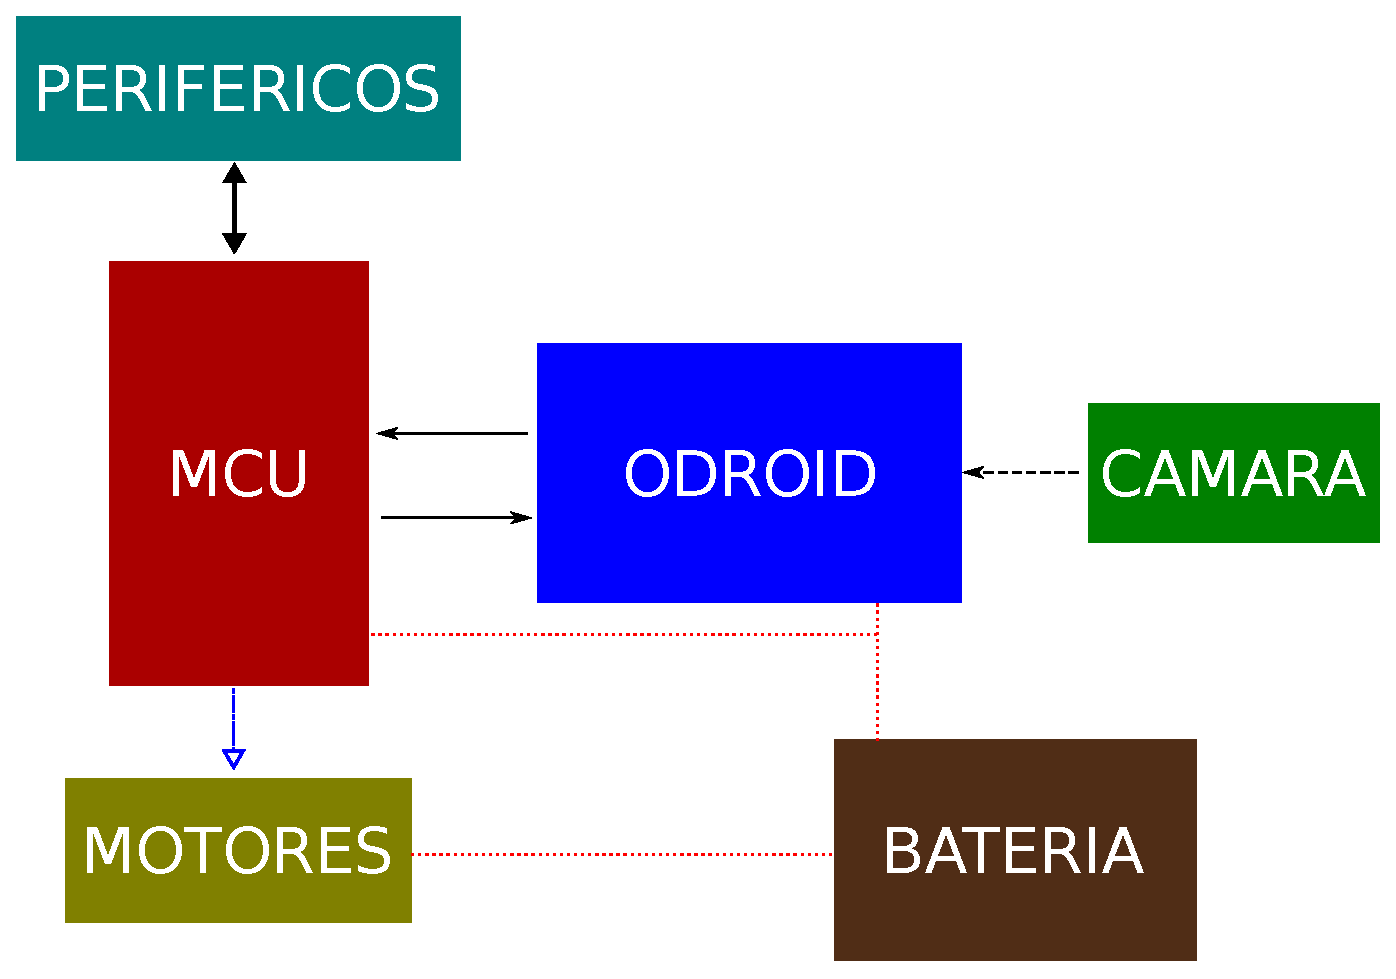
\includegraphics[width=0.5\textwidth]{Contenido/Cuerpo/Capitulo5/Fig13.eps}
	\captionof{figure}{Arquitectura del sistema}\label{Fig1}
\end{center}
El microcontrolador es de 32 bits arquitectura RISC, las especificaciones detalladas de los motores y de la tarjeta de desarrollo
ODROID puede ser consultada en el Apéndice B.\\
El Bus señalado con líneas punteadas en rojo representan la conexión de voltaje con los demás componentes, mientras que la línea punteada en negro entre la cámara y la odroid
simboliza la conexión USB para la transferencia de datos, la comunicación entre ODROID y el MCU se da mediante el módulo RS-323 integrado en el microcontrolador que a su vez
se comunica con los periféricos deseados utilizando sus salidas digitales.\\
Este tipo de Arquitectura permite que la ODROID pueda comunicarse paralelamente con el MCU por medio del protocolo serial, que va
a 57000 baudios, además de que permite que el microcontrolador tenga la posibilidad de publicar en ROS.

% ---------------------------------------------------------------------------------------------------------
% *********************************************************************************************************
% *********************************************************************************************************
% ---------------------------------------------------------------------------------------------------------


\section{Mecanismo móvil}
El diseño del sistema fue hecho con un programa de uso de software libre llamado OpenSCAD, en el cual se trazó el prototipo del
sistema utilizando dos motores tipo servo, es decir, que tienen su propio controlador de velocidad integrada vía PWM.
\begin{center}
	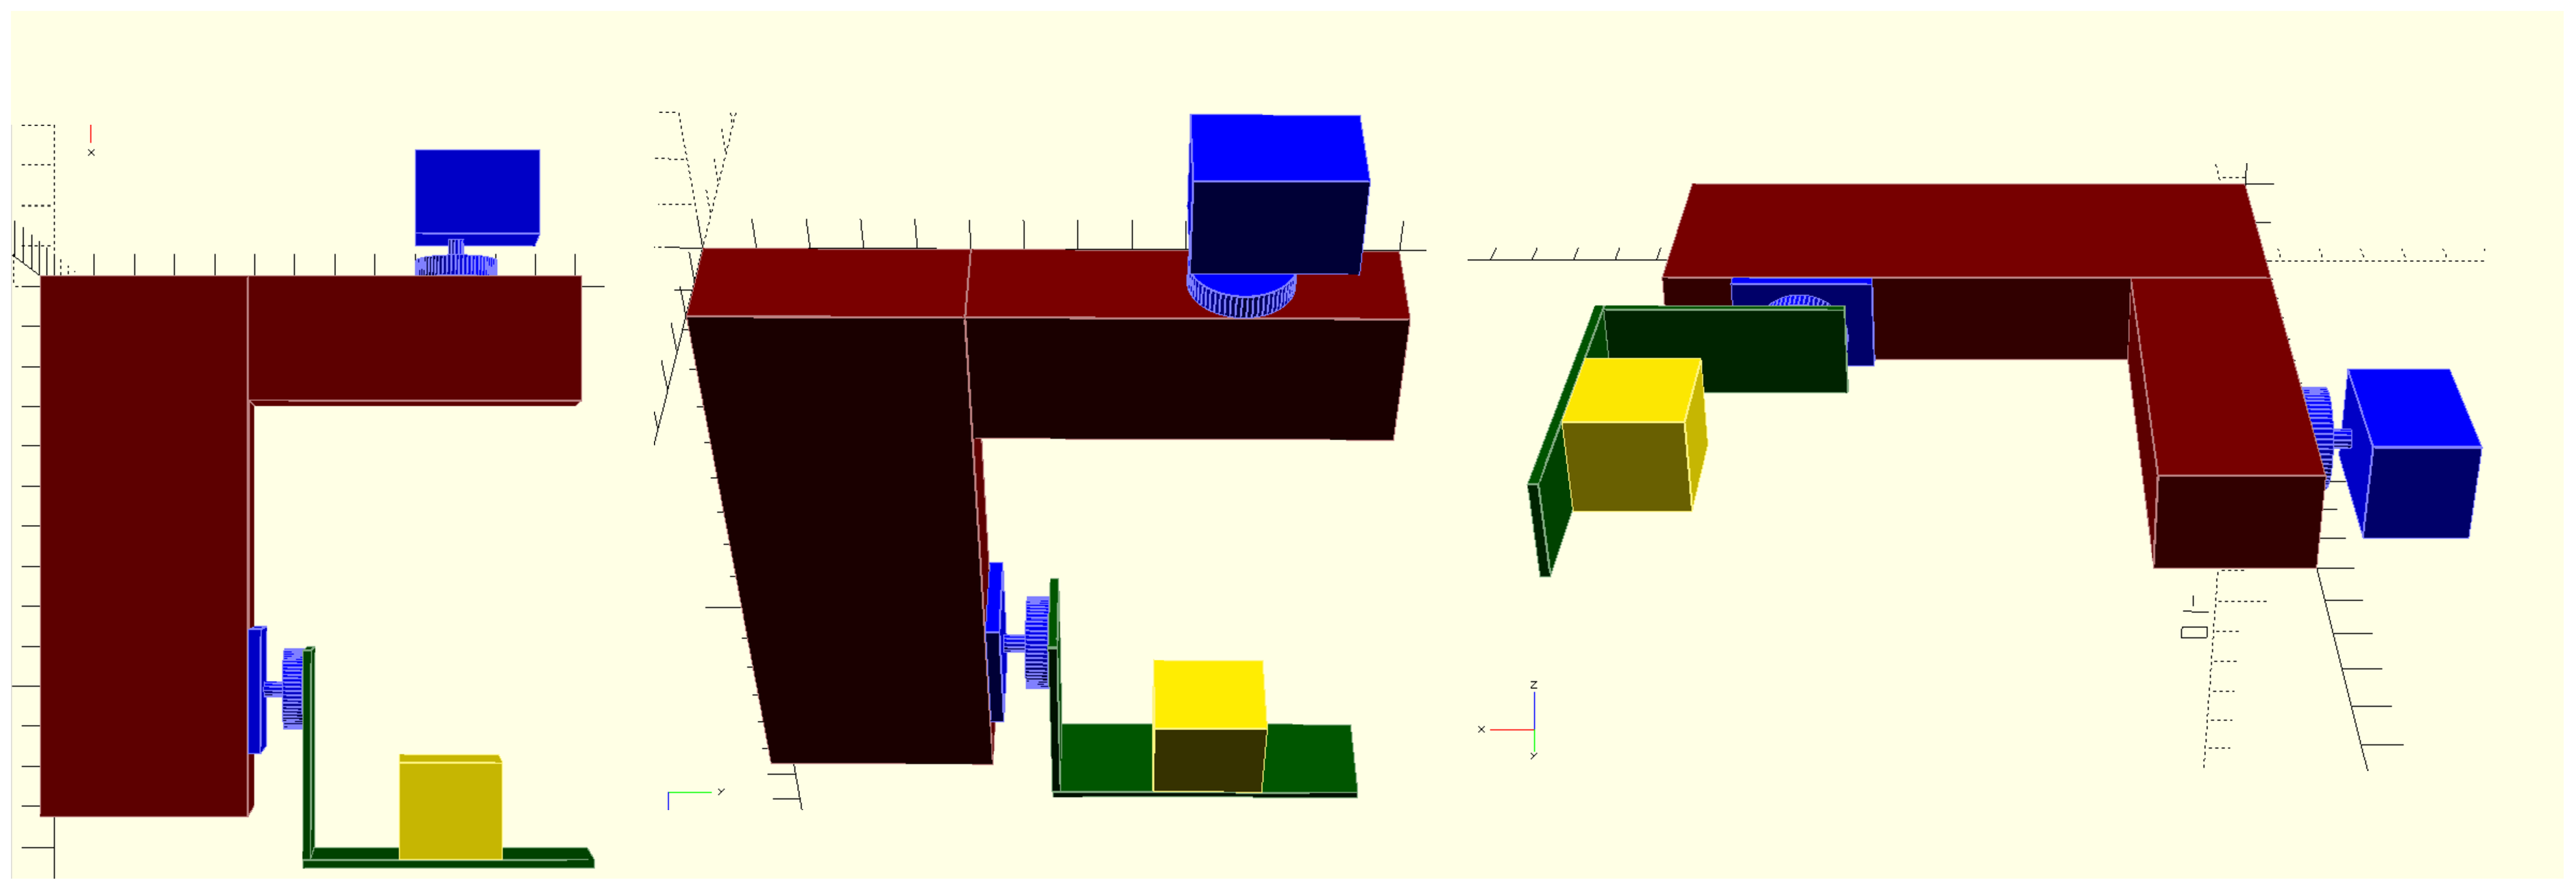
\includegraphics[width=1.0\textwidth]{Contenido/Cuerpo/Capitulo5/Fig14.eps}
	\captionof{figure}{Diseño CAD del prototipo}\label{Fig1}
\end{center}
En la figura 5.3 los motores están representados en color azul, mientras que la cámara esta de amarillo, como se puede apreciar
la cámara recae sobre un soporte de color verde, dicha cámara está sujeta por un par de ligas que ayudan a que esta no se
caiga cuando hay rotación en pitch.\\
A continuación en la figura 5.4 se presentan algunas medidas del diseño, las unidades están en mm.
\begin{center}
	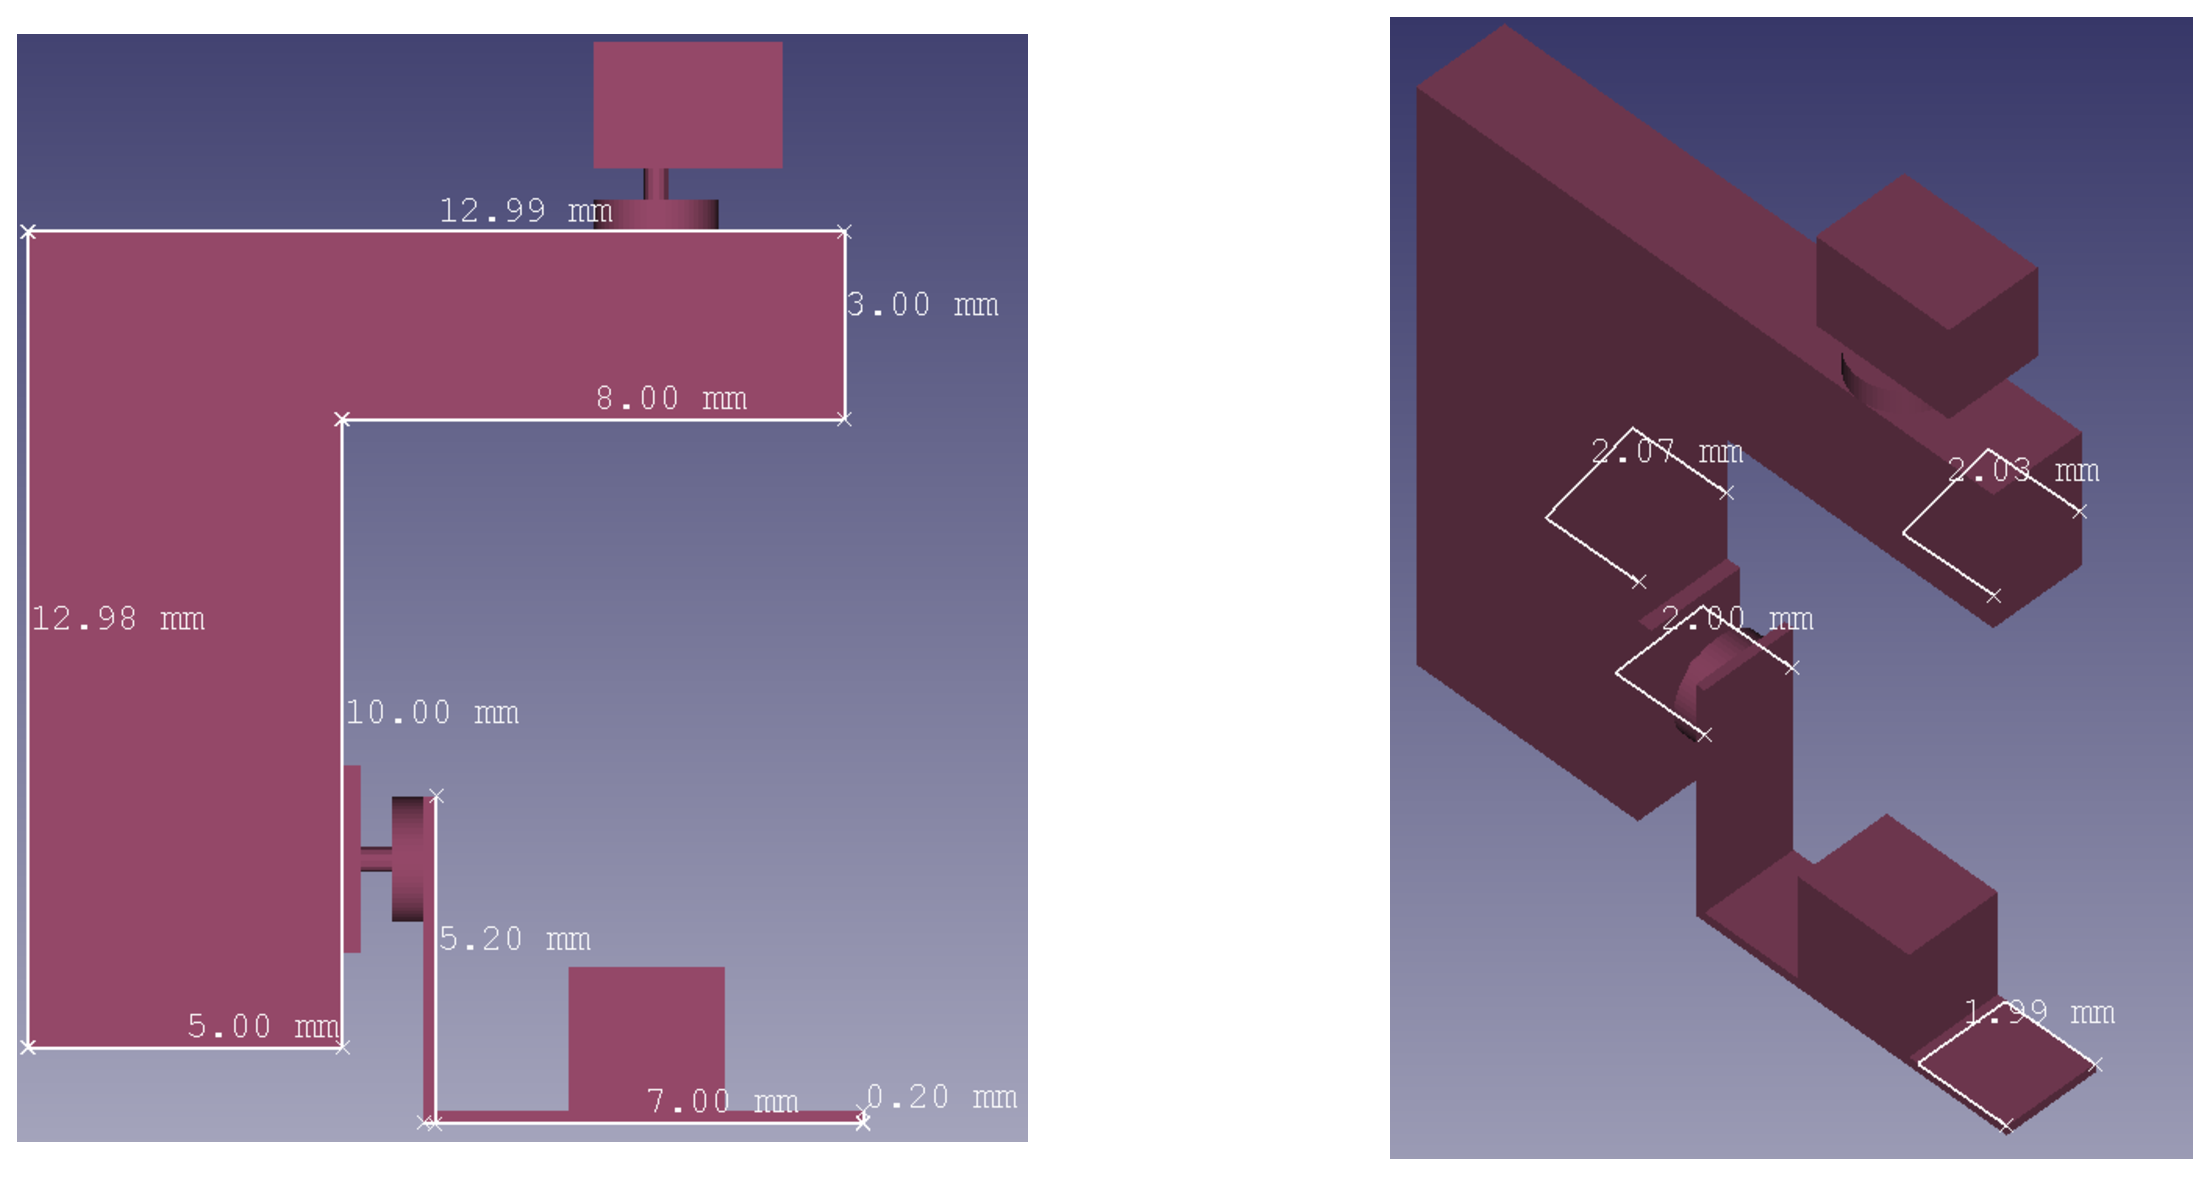
\includegraphics[width=0.8\textwidth]{Contenido/Cuerpo/Capitulo5/Fig16.eps}
	\captionof{figure}{Dimensiones del CAD}\label{Fig1}
\end{center}
Como se vio previamente en los capítulos 2 y 3 este sistema tendrá dos ejes de libertad, que en términos técnicos, a estos
movimientos también se les conoce como "\ Till "\ para los movimientos pitch y "\ Pan "\ para movimientos en yaw que es no es mas que otra manera de decirle a la rotación
sobre el eje Y y Z.\\
Es entonces que esos movimientos pueden ser visualizados como se presenta en la figura 5.5.
\begin{center}
	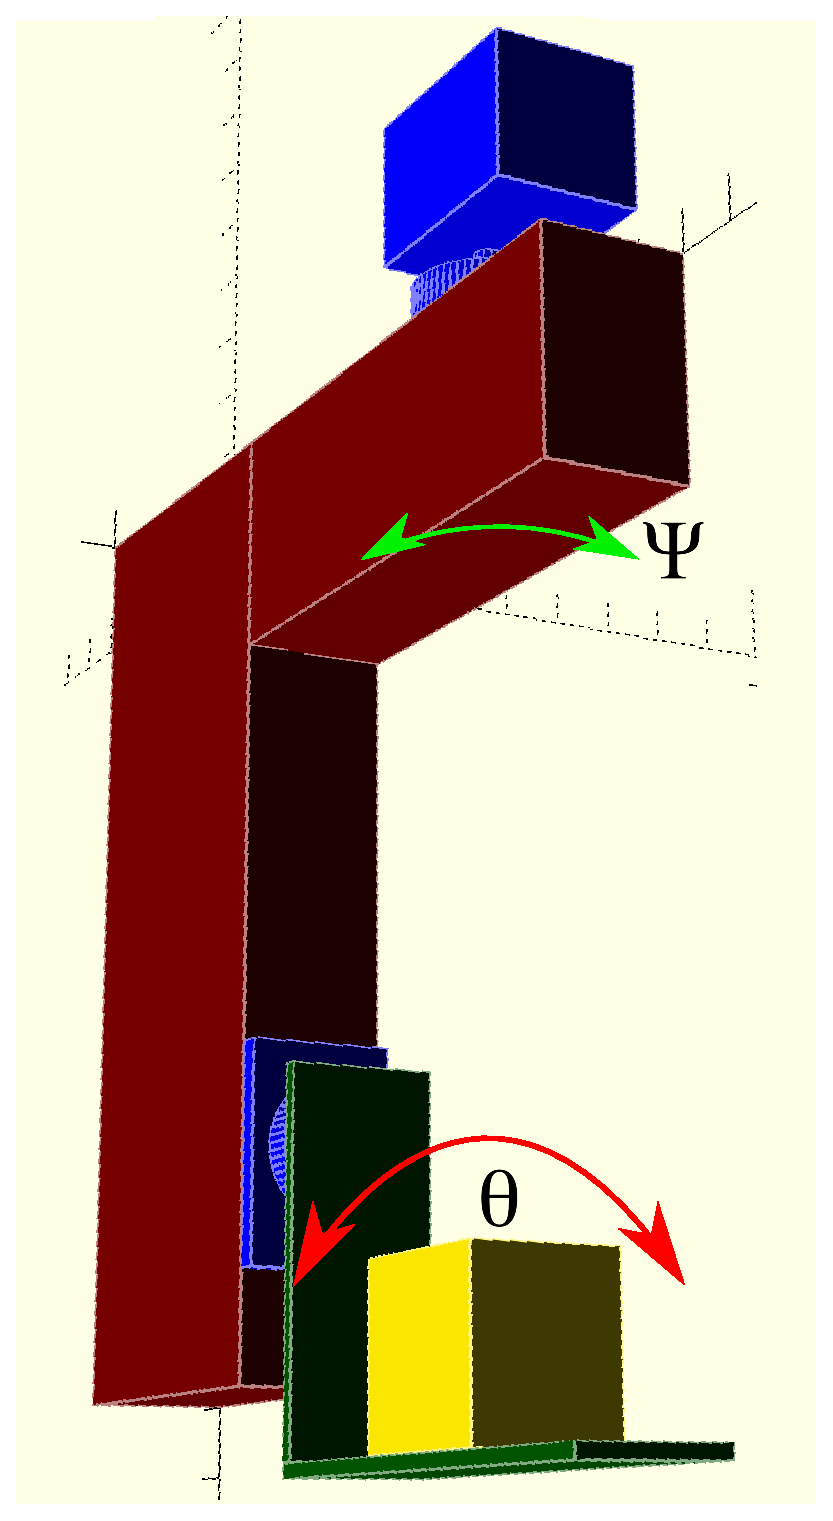
\includegraphics[width=0.35\textwidth]{Contenido/Cuerpo/Capitulo5/Fig15.eps}
	\captionof{figure}{Grados de libertad del sistema}\label{Fig1}
\end{center}
Donde
\begin{itemize}
	\item $\theta$ representa el movimiento de "\ Till "
	\item $\psi$ representa el movimiento de "\ Pan  "
\end{itemize}

% ---------------------------------------------------------------------------------------------------------
% *********************************************************************************************************
% *********************************************************************************************************
% ---------------------------------------------------------------------------------------------------------
\section{Prototipo físico}
Para la realización del prototipo se utilizó un material ligero para que no agregue mucho peso adicional al sistema.
\begin{center}
	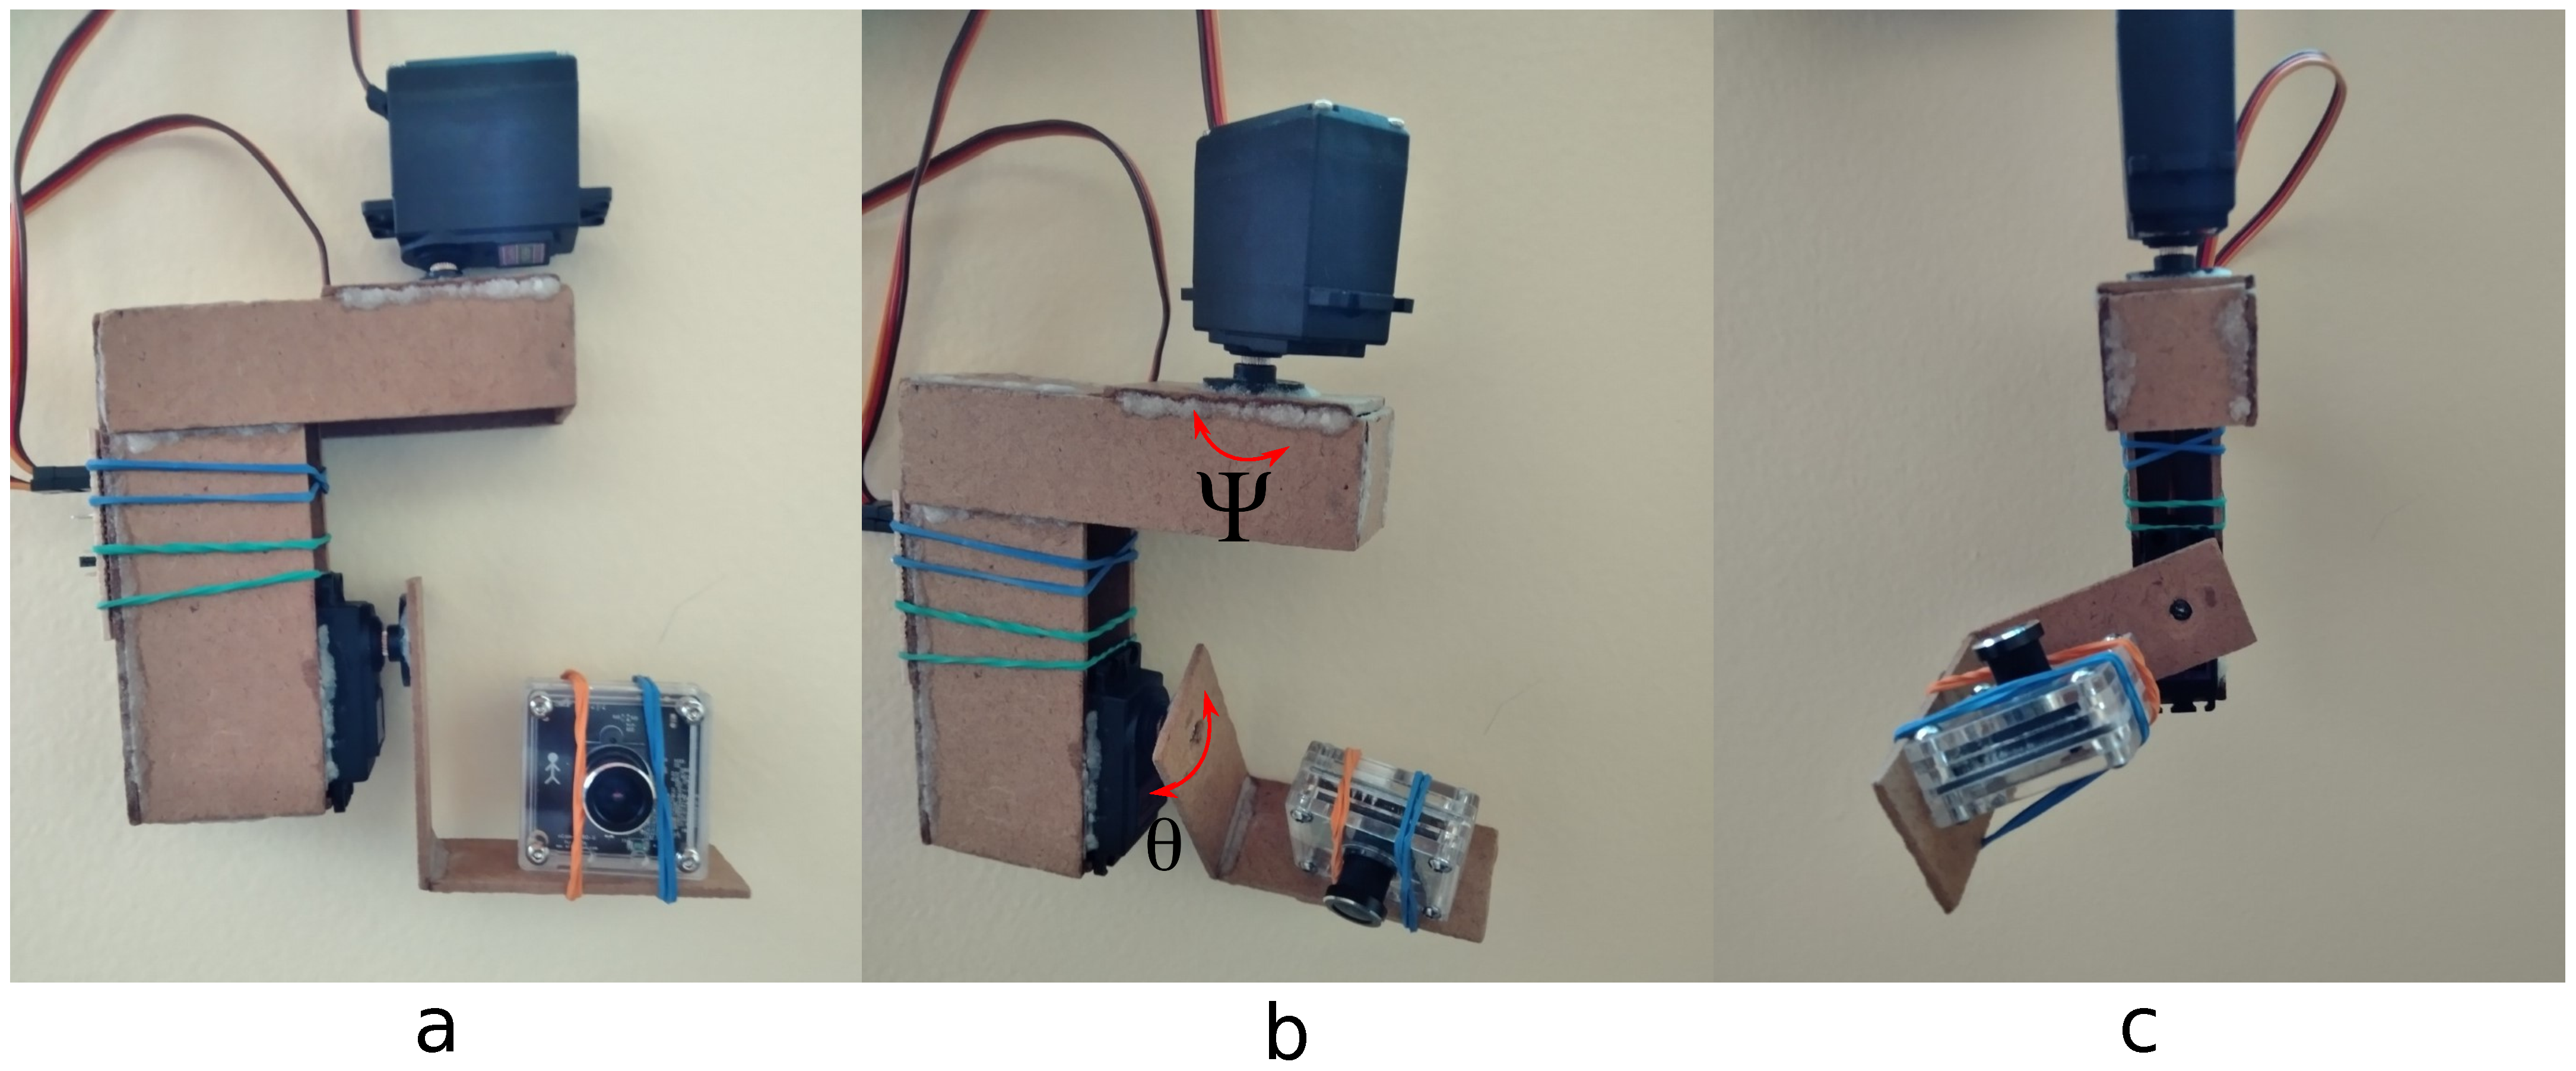
\includegraphics[width=0.8\textwidth]{Contenido/Cuerpo/Capitulo5/Fig17.eps}
	\captionof{figure}{Prototipo del sistema hecho con madera}\label{Fig1}
\end{center}
Como se puede observar en la figura 5.6 la cámara esta sujeta a la base por medio de ligas que le dan mejor soporte y ayudan a que
esta no se caiga al momento de seguir a los objetivos.
\begin{itemize}
    \item Peso del sistema sin motores ni cámara: 70 g
    \item Peso con motores y cámara: 215 g
\end{itemize}
En b) y c) de la figura 5.6 se ilustra el movimiento que puede realizar el sistema, y que será controlado
por la cámara y actuado por los motores.
\begin{center}
	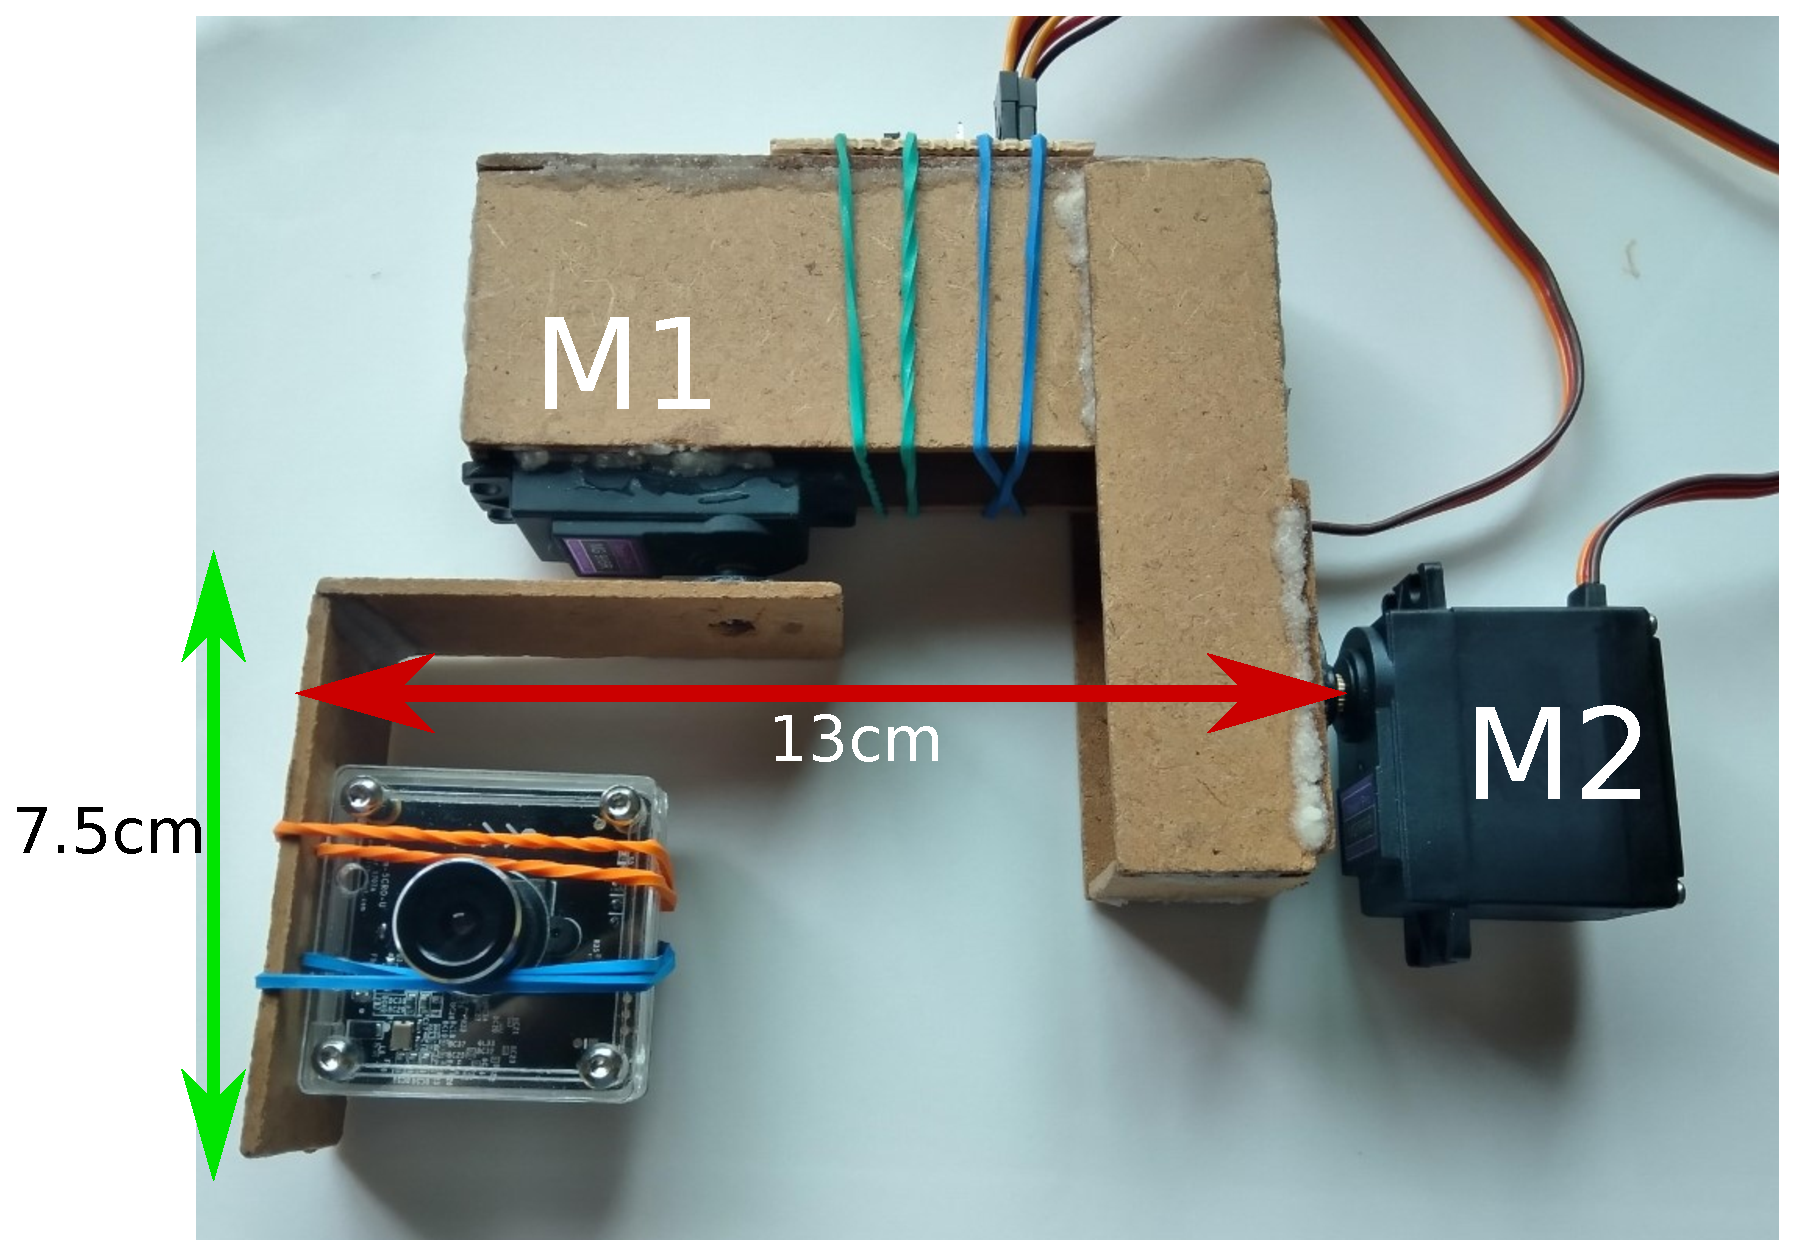
\includegraphics[width=0.6\textwidth]{Contenido/Cuerpo/Capitulo5/Fig20.eps}
	\captionof{figure}{Vista frontal del prototipo}\label{Fig4}
\end{center}
Adicionalmente se diseñó un pequeño circuito que sirve como terminal para las conexiones de alimentación y señales,
dicho circuito se encuentra en la parte lateral del sistema sujetado por ligas y pegamento.\\
La conexiones eléctricas se ilustra en la figura 5.8. Es un esquemático que muestra la conexión entre los componentes principales: la cámara(OCAM), monoprocesador(ODROID),
el microcontrolador (ATMEGA, ver características en apéndice B) y los motores (Servomotores).
\begin{center}
	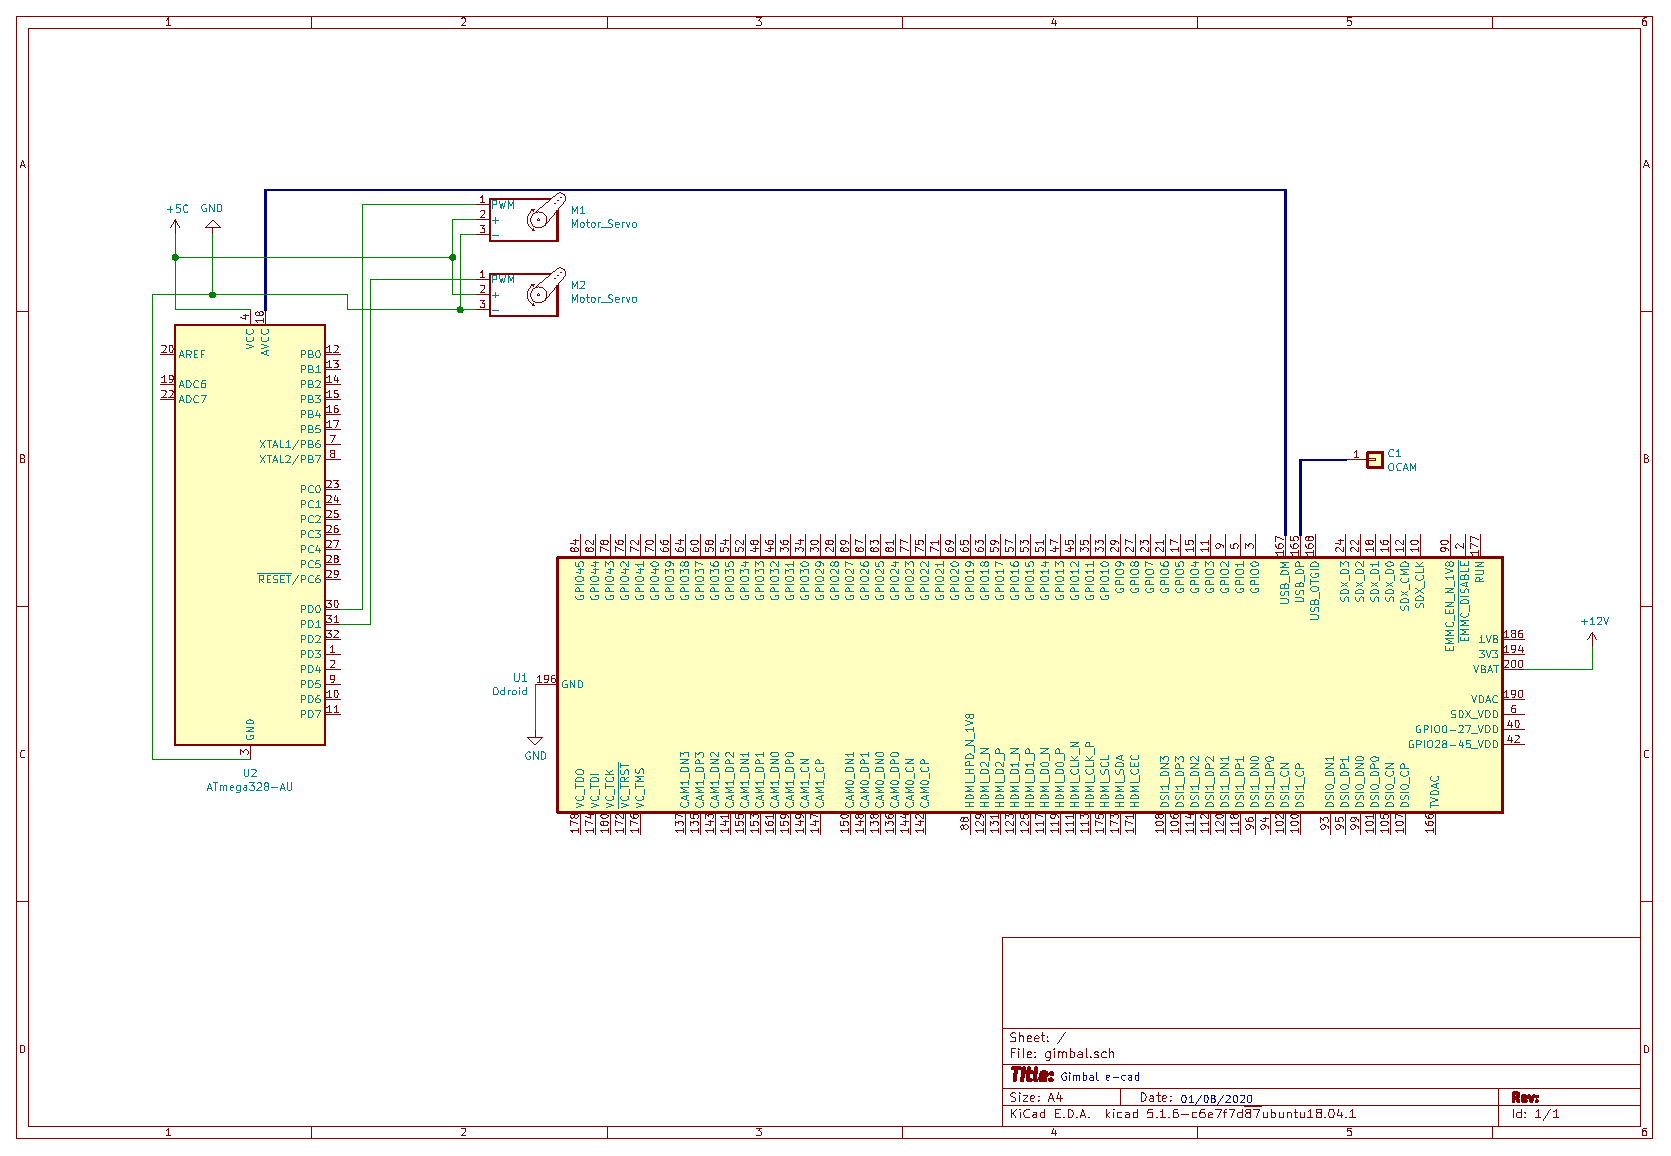
\includegraphics[width=1.0\textwidth]{Contenido/Cuerpo/Capitulo5/Fig21.eps}
	\captionof{figure}{Circuito eléctrico}\label{Fig1}
\end{center}


% ---------------------------------------------------------------------------------------------------------
% *********************************************************************************************************
% *********************************************************************************************************
% ---------------------------------------------------------------------------------------------------------


\section{ROS-Microcontrolador}
La parte mecánica encargada de hacer mover la cámara alrededor de dos ejes son los motores de corriente directa, que están conectados
a un microcontrolador que es el encargado de ejecutar el controlador.\\
El control tiene como entrada las coordenadas obtenidas por el algoritmo descrito en el capítulo 4. Y con base en ese píxel, podemos
calcular el error teniendo en cuenta que la referencia es el centro de la cámara.\\
Una vez dicho lo anterior queda una pregunta clara, ¿Como comunicar el microcontrolador encargado de los motores, con la cámara que
está siendo ejecutada en ROS?.
\begin{center}
	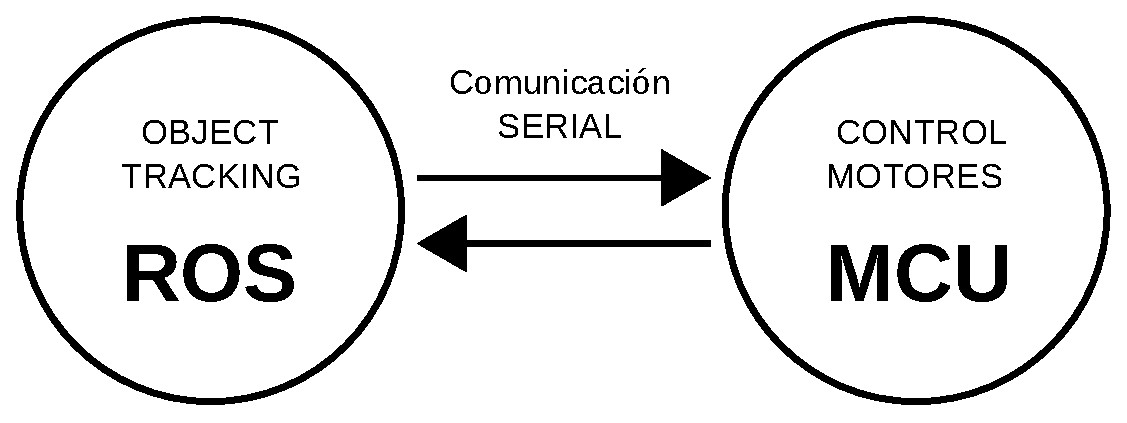
\includegraphics[width=0.55\textwidth]{Contenido/Cuerpo/Capitulo5/Fig1.eps}
	\captionof{figure}{Protocolo de comunicación}\label{Fig2}
\end{center}
Como se ilustra en la imagen 5.9 el protocolo de comunicación que se utilizó es el serial, debido a su practicidad y que ya
cuenta con librerías de ROS para el microcontrolador, que para la primera etapa de esta investigación se utiliza el Atmega328p.\\
La comunicación está basado en ser asíncrona, y se detalla mejor diagrama 5.10.
\begin{center}
	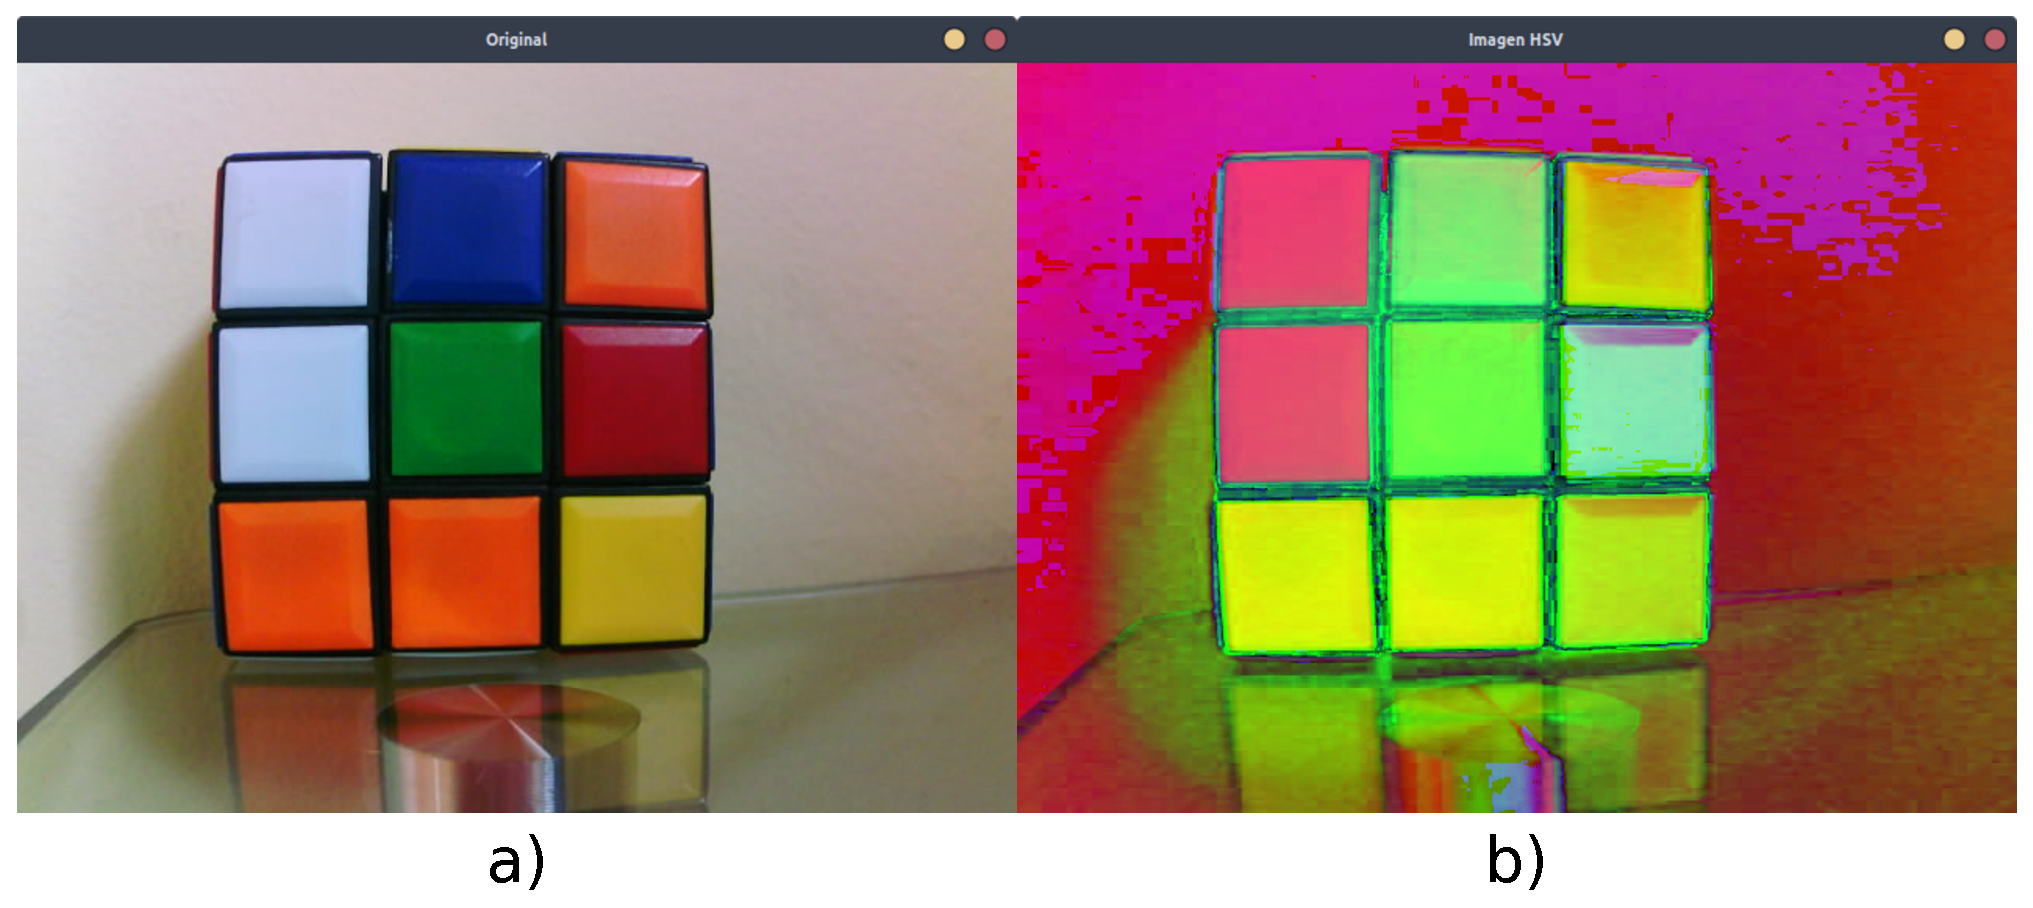
\includegraphics[width=0.45\textwidth]{Contenido/Cuerpo/Capitulo5/Fig2.eps}
	\captionof{figure}{Diagrama de secuencia}\label{Fig3}
\end{center}
La velocidad de la comunicación es de 570000 baudios y se conecta a través de un cable usb. El microcontrolador tiene además
la función de publicar el error con la finalidad de graficar dicho error y obtener conclusiones. Que visto desde el plano
de ROS tenemos los siguientes Tópicos y Nodos:
\begin{center}
	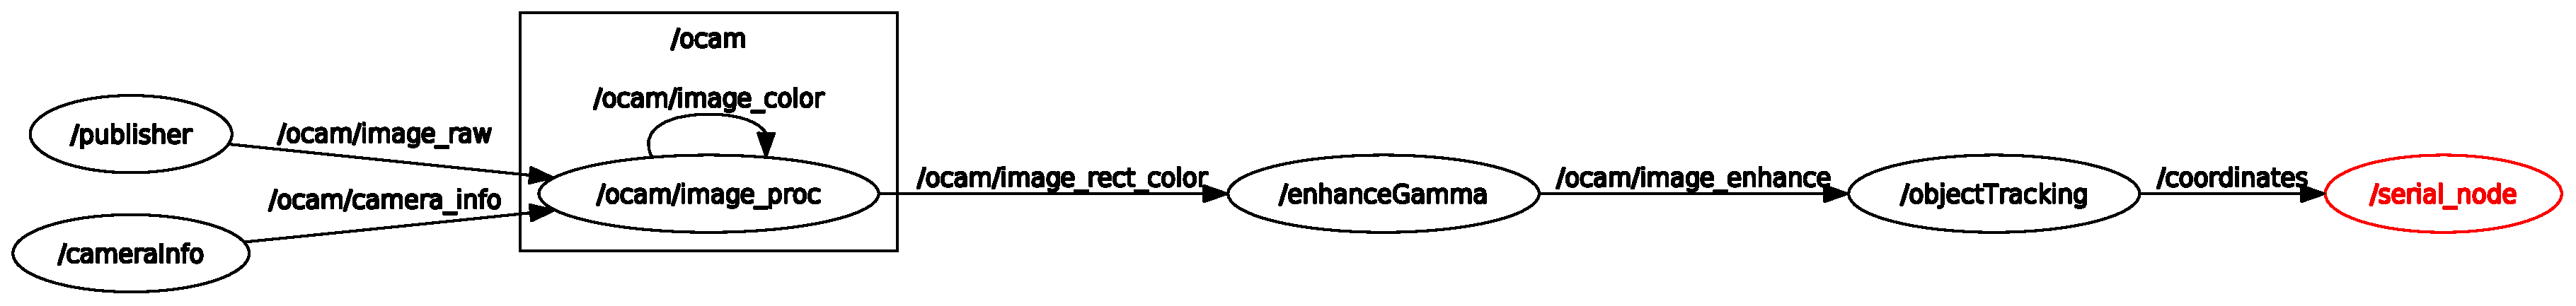
\includegraphics[width=1.0\textwidth]{Contenido/Cuerpo/Capitulo5/Fig3.eps}
	\captionof{figure}{Nodos y Tópicos activos}\label{Fig4}
\end{center}


% ---------------------------------------------------------------------------------------------------------
% *********************************************************************************************************
% *********************************************************************************************************
% ---------------------------------------------------------------------------------------------------------


\section{Control}
La idea principal del sistema de control es la de encontrar una función de entrada $u(t)$ tal que la función de salida $x(t)$ siga a la
salida deseada $x^{des}(t)$. Es decir la diferencia entre la salida deseada y la actual, tal y como se expresa en la ecuación 5.1.
\begin{equation}
	e(t) = x^{des}(t) - x(t)
\end{equation}
Donde $e(t)$ representa el error. Por lo que la estrategia es encontrar un $u(t)$ tal que
\begin{equation}
	K_i\int e + k_pe = 0
\end{equation}
Donde $k_i$ y $k_p$ $> 0$\\
La ecuación 5.2 representa un controlador proporcional-integral que se verá más a detalle a lo largo de este capítulo, la ec 5.3 se define el control en el tiempo.
\begin{equation}
	u(t) = k_i\int{e}(t) + k_pe(t)
\end{equation}

% \subsection{Control servomotor}
% Como vimos en el capítulo 3, la función de transferencia de un motor de corriente continua es de segundo orden ec 5.4, e involucra algunas constantes que dependen del toque máximo y
% de la velocidad sin carga.
% \begin{equation}
	% \frac{\theta_m (s)}{E_a(s)} = \frac{K_t / (R_aJ_m)}{s \left[ s + \frac{1}{J_m} \left( D_m + \frac{K_tK_b}{R_a} \right) \right]}
% \end{equation}
% El motor que se utilizó para hacer el mecanismo móvil es el MG996R, es un motor de tipo servo 360 grados, a diferencia de los servomotores
% convencionales que solo son de 180° este no permitirá hacer un control de posición con base en el error antes descrito. Las especificaciones técnicas son las siguientes:
% \begin{itemize}
	% \item Peso = 55g
	% \item Torque stall = 11kg/cm a 6v
	% \item Velocidad sin carga = 0.14s/ 60° a 6v
	% \item Voltaje de operación = 4.8v a 7.2v
	% \item Temperatura de operación = 0°C - 55°C
	% \item PWM = 20ms (50Hz) de operación
% \end{itemize}
% La gráfica 5.11. muestra la relación que hay entre el torque y la velocidad, que como se puede observar es lineal. Esta grafica se obtuvo con los datos sugeridos del
% provedor.
% \begin{center}
	% 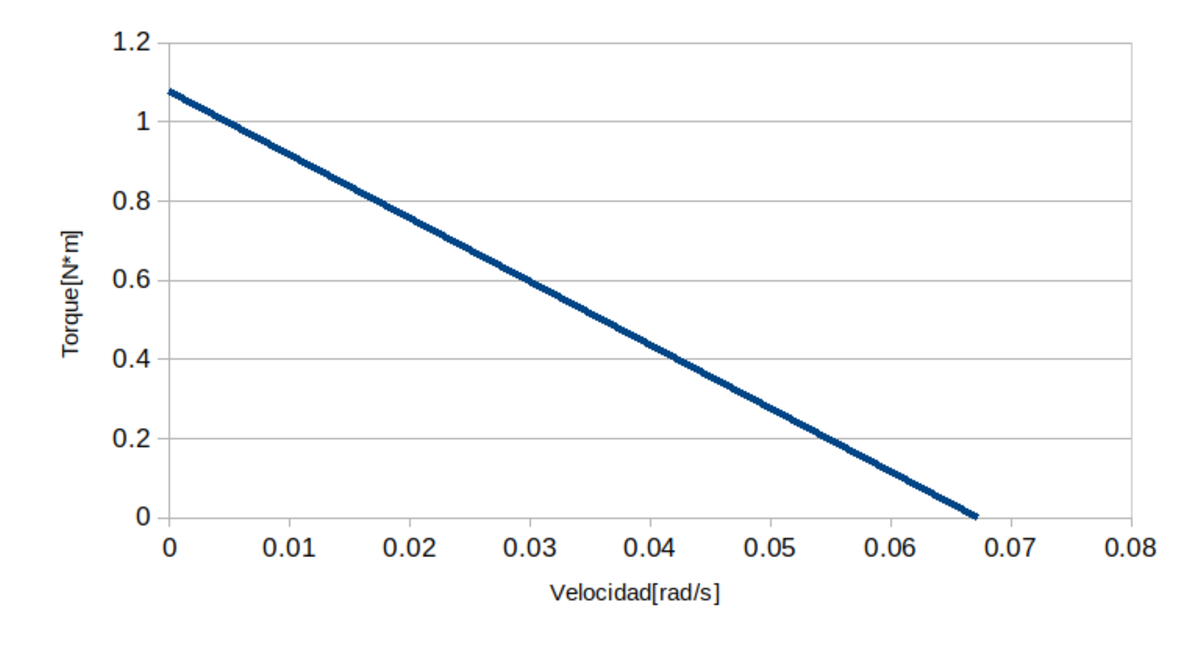
\includegraphics[width=0.8\textwidth]{Contenido/Cuerpo/Capitulo5/Fig19.eps}
	% \captionof{figure}{Gráfica torque-velocidad}\label{Fig4}
% \end{center}
% Este servomotor como la mayoría en el mercado cuenta con su propio lazo de control, lo que hace que el sistema tenga como limitante la velocidad de respuesta del motor.
% En el capítulo 3 se definieron las ecuaciones dinámicas para los movimientos en pitch y yaw, de donde la entrada viene dada por un porque en el eje z ($T_k$) y en el eje y ($T_y$)
% para este proyecto vamos a tomar los motores como entradas de porque, es decir, que se mueven hacía la posición que el controlador requiera, clara con su debido tiempo de
% respuesta propia del controlador interno del motor.



\subsection{Control en Pitch}
El sistema dinámico de Pitch obtenida en el capítulo 3 se trata de una ecuación de primer orden
\begin{equation}
	J_{ay}\dot{q}_a = T_y
\end{equation}
Pasando la ecuación 5.5 al dominio de Laplace, obtenemos
\begin{equation}
	J_{ay}SQ_a(s) = T_y(s)
\end{equation}
Dividimos entrada entre salida, o en otras palabras, obtenemos la función de transferencia en lazo abierto
\begin{equation}
	G = \frac{Q_a(s)}{T_y(s)} =  \frac{1}{J_{ay}s}
\end{equation}
Y en lazo cerrado la ecuación 5.7 se transforma en
\begin{equation}
	G_c = \frac{G}{1 +GH} = \frac{1}{J_{ay}s+1}
\end{equation}
La figura 5.13 es el resultado de la simulación del sistema dinámico de pitch en lazo cerrado en respuesta a una entrada escalón.
\begin{center}
	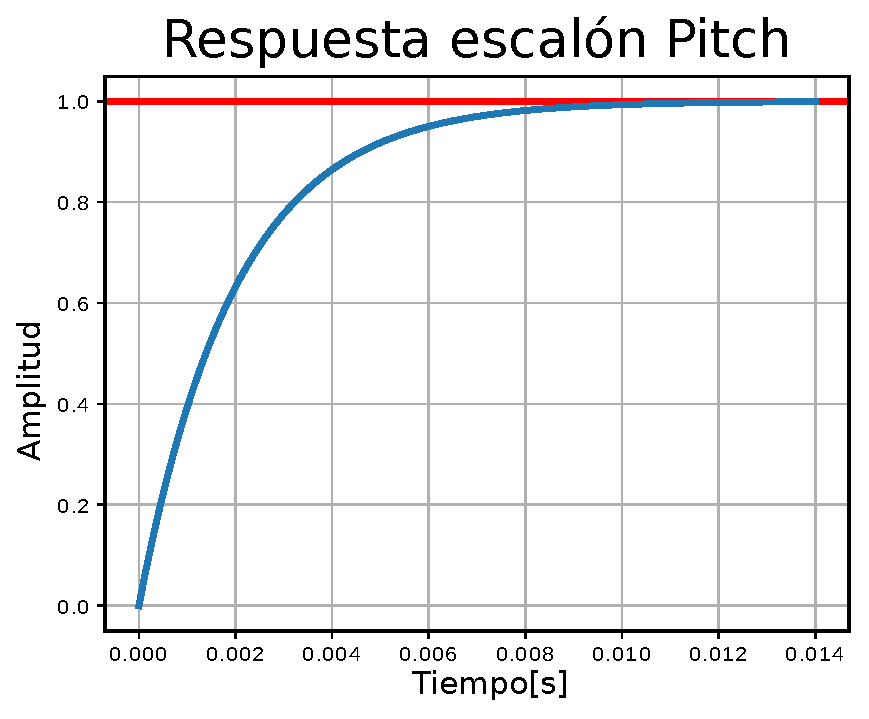
\includegraphics[width=0.7\textwidth]{Contenido/Cuerpo/Capitulo5/Fig35.eps}
	\captionof{figure}{Simulación entrada escalón}\label{Fig4}
\end{center}
Los valores para la ecuación 5.14 se obtuvieron del trabajo de \cite{Paper::Abdo2013}, debido a la similitud del sistema físico, donde
$J_{ay} = 0.002$

Como se abordó en el capítulo 3, el sistema dinámico de la gimbal es de primer orden para los movimientos en pitch y yaw, y como se introdujo en la sección 5.5
el control que se implementó es el Proporcional-Integral. Siendo este el necesario para hacer que el error converja a cero.\\
El diagrama de bloques de la figura 5.14 une todas las etapas de control, pasando por el control del servomotor, que hace una retroalimentación interna con base
en la dinámica vista en la sección 5.1 y que obtenemos como salida el porqué de entrada de la función de transferencia de la dinámica de Pitch para posteriormente
obtener la velocidad angular $q_a$, que después pasa por un integrador y así obtener la posición respecto al marco de referencia de la cámara, es decir, en
píxeles de la coordenada Y.
\begin{center}
	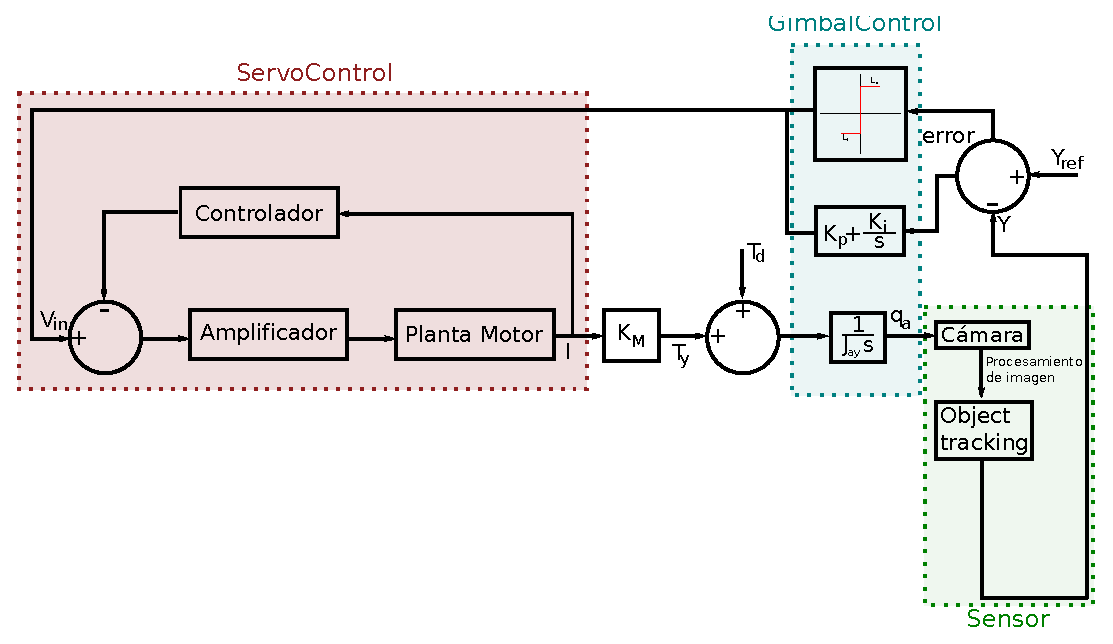
\includegraphics[width=1.0\textwidth]{Contenido/Cuerpo/Capitulo5/Fig22.eps}
	\captionof{figure}{Lazo de control para Pitch}\label{Fig4}
\end{center}
% Es un sistema de segundo orden retroalimentado por la camara y procesado en ROS. El lazo de control es aplicable también para la coordenada Y, como
% fue abordado en la sección 5.4 la comunicación se da mediante
% el protocolo serial, y debido a que la tarea que se encarga de realizar el algoritmo de control se debe suscribir al nodo de
% coordenadas, este se ve limitado, a un tiempo de muestreo de 60fps, o dicho de otro modo a 16.66 ms.

\subsubsection{Diseño de controlador}
El sistema tiene un controlador PI, donde tenemos la acción proporcional al error, que se encarga de acelerar la respuesta del sistema para llegar a la referencia
y tendrá la acción integradora que se encarga de ajustar automáticamente el BIAS integrando el área bajo la curva del error presente en el proceso y de esa forma
eliminar el error en estado estacionario. Tenemos que la función de transferencia del controlador PI viene dado por la expresión 5.9.
\begin{equation}
	C(s) = Kp(1 + \frac{1}{T_is})
\end{equation}
Donde $K_p$ es la ganancia proporcional y $T_i$ es el tiempo integral. La técnica para el diseño del control se llama asignación de polos.\\
Aplicamos el lazo cerrado a la planta con el controlador, es decir $G_c(s) = G(s)C(S)$
\begin{equation}
	G_c(s) = \frac{500K_ps + \frac{500K_p}{T_i}}{s^2 + 500K_ps + \frac{500K_p}{T_i}}
\end{equation}
De donde obtenemos la ecuación característica 5.11
\begin{equation}
	E.C_1 = s^2 + 500K_ps + \frac{500K_p}{T_i}
\end{equation}
Como todavía no hemos definido cuáles serán los parámetros del controlador PI, estos nos servirán para ubicar los polos en el lugar que nosotros queremos, es por
eso que esta técnica es conocida como asignación de polos.\\
Como condiciones de diseño tenemos que considerar lo siguiente:
\begin{itemize}
	\item El sistema teóricamente podría establecerse en un tiempo de 0.01 segundos acorde a la figura 5.13, sin embargo físicamente no es posible debido a dos
		factores, los motores ya tienen su lazo de control incluido como se detalló en la sección 5.5.1 y la velocidad sin carga es de 0.14s lo cual es una
		limitante y segundo el tiempo de muestreo de la cámara es mayor al de establecimiento del control, ya que está en 60Hz.
	\item Por lo anterior el tiempo de asentamiento $T_s$ se establece en 0.2s 
	\item El porcentaje de error se establece en 2\%
	\item Y el pico Máximo $M_p$ no debe pasar del 2\%
\end{itemize}
La función deseada que cumpla los puntos anteriores es de la forma 
\begin{equation}
	G_d(s) = \frac{\omega_n^2}{s^2 + 2\zeta\omega + \omega_n^2}
\end{equation}
Donde el factor de amortiguamiento está dado por
\begin{equation}
	\zeta = \sqrt{\frac{\ln\left(\frac{M_p}{100}\right)^2}{\pi^2 + \ln\left(\frac{M_p}{100}\right)^2}}
\end{equation}
Y la frecuencia natural viene dada por la expresión 5.14
\begin{equation}
	\omega_n = \frac{3}{\zeta T_s}
\end{equation}
A partir de las ecuaciones 5.13 y 5.14 y con los parámetros de diseño obtenemos la función de transferencia con los polos deseados 
\begin{equation}
	Gd(s) = \frac{1086}{s^2 + 60s + 1086}
\end{equation}
La ecuación característica de la función de transferencia de la ecuación 5.15 viene dada por la
expresión 5.16
\begin{equation}
	E.C_2 = s^2 + 60s + 1086 = s^2 + \alpha_1s + \alpha_2
\end{equation}
Donde los polos deseados se sitúan en $s_{1,2} = -30, \pm 13.6437j$ \\
Igualamos la ecuación 5.11 con 5.16 para calcular el valor de $K_p$ y $T_i$
\begin{equation}
	500K_p = \alpha_1
\end{equation}
\begin{equation}
	\frac{500K_p}{T_i} = \alpha_2
\end{equation}
A partir de las ecuaciones 5.17 y 5.18 obtenemos los valores de $K_p = 0.118$ y $T_i = 0.054$, por lo que nuestro controlador viene dado por la ecuación 5.19.
\begin{equation}
	C(s) = 0.118 + \frac{2.1851}{s}
\end{equation}
El diagrama de la figura 5.15 muestra el lazo cerrado de controladorPI y la planta para el movimiento en pitch
\begin{center}
	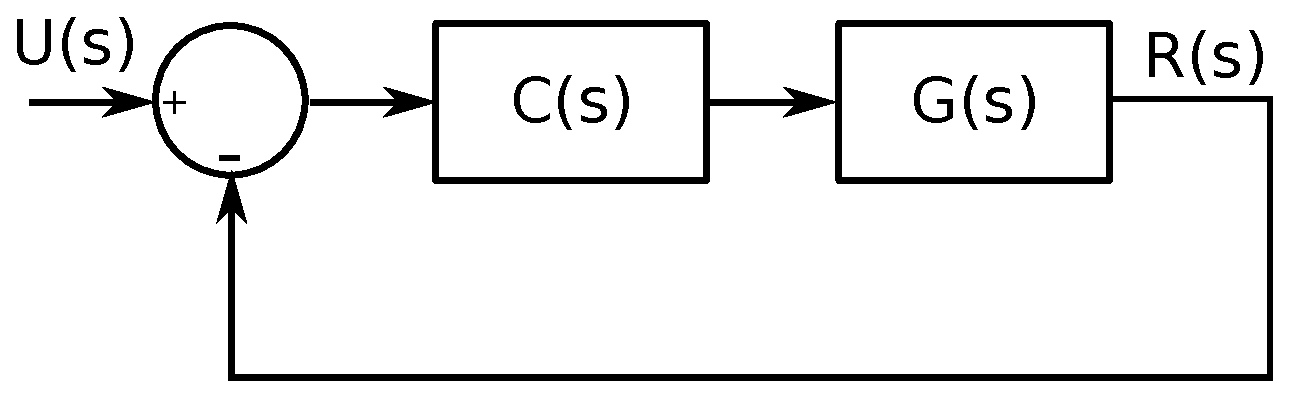
\includegraphics[width=0.6\textwidth]{Contenido/Cuerpo/Capitulo5/Fig37.eps}
	\captionof{figure}{Lazo cerrado del sistema con control PI}\label{Fig4}
\end{center}
Si aplicamos U(s) = 1, obtenemos la siguiente respuesta en el tiempo del sistema. 
\begin{center}
	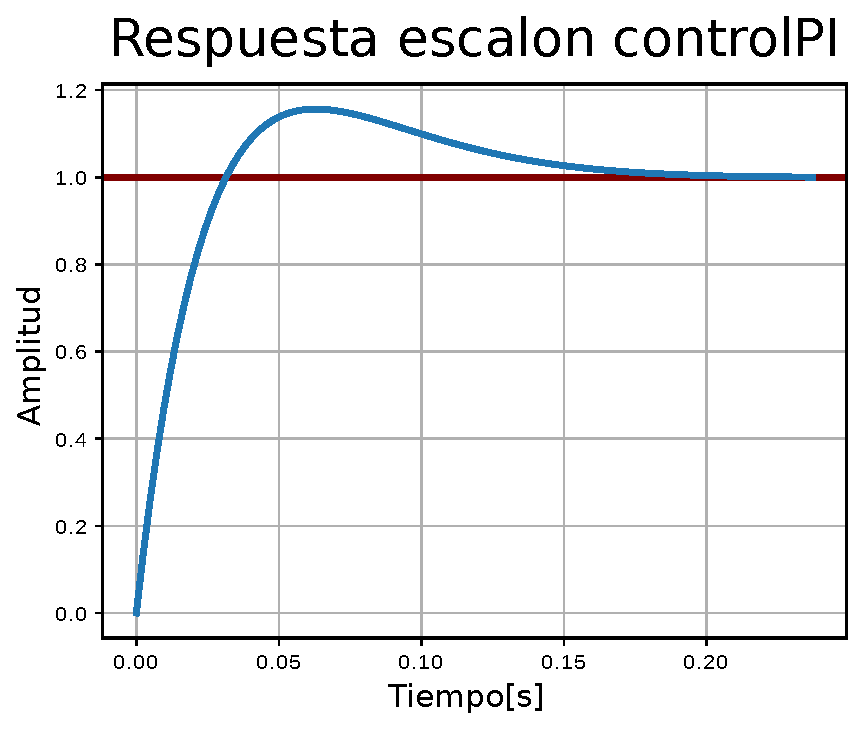
\includegraphics[width=0.6\textwidth]{Contenido/Cuerpo/Capitulo5/Fig38.eps}
	\captionof{figure}{Simulación respuesta escalón en pitch}\label{Fig4}
\end{center}
La simulación de la figura 5.16 muestra que el sistema tiene un tiempo de establecimiento de 0.2 segundos tal y como se
planeó en la etapa de diseño, hay un pequeño sobre impulso que en la práctica no representara más del 2\%. El código para
la simulación está hecho en python y puede ser consultado en mi repositorio de \href{https://github.com/MarcoAAG/Tesis}{\textbf{GitHub}}.
La Ganancia Ki de la ecuación 5.25 se ve modificada en el microcontrolador debido a que se utiliza el método numérico para la integración del error, por lo que
la ganancia se multiplica por el tiempo de muestreo que es de 0.016, entonces la ecuación 5.25 se convierte en:
\begin{equation}
	C(s) = 0.118 + \frac{0.034}{s}
\end{equation}
\subsubsection{Algortimo de control}
El algoritmo general del control tanto para pitch y para yaw está descrito en el diagrama 5.17, basado en programación orientado a objetos
donde hay dos puntos claves, la obtención de datos de la cámara vía serial y la publicación de los errores para su posterior uso en gráficas.
\begin{center}
	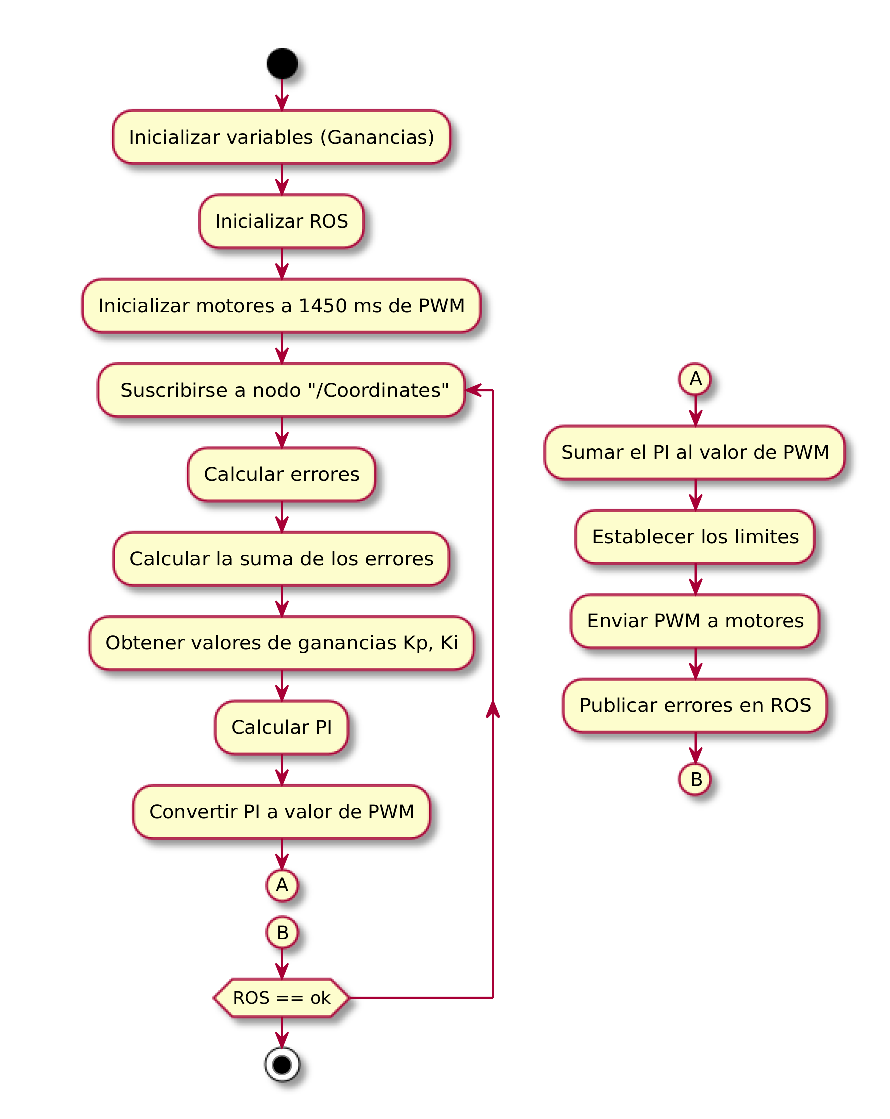
\includegraphics[width=0.6\textwidth]{Contenido/Cuerpo/Capitulo5/Fig24.eps}
	\captionof{figure}{Diagrama de flujo de algoritmo de control}\label{Fig4}
\end{center}
\subsubsection{Sintonización de control}
Lo primero que se realizó fue un controlador proporcional y se analizó su respuesta en el tiempo, de la cual se graficó el error, teniendo
como referencia el cero.\\
La figura 5.18 muestra el resultado de sintonizar la ganancia Kp a uno, como se puede observar el sistema comienza en las primeras 50 muestras
para después dar paso a un reposo, el error se mantiene en 20, por lo que el siguiente paso fue reducir la ganancia Kp
\begin{center}
	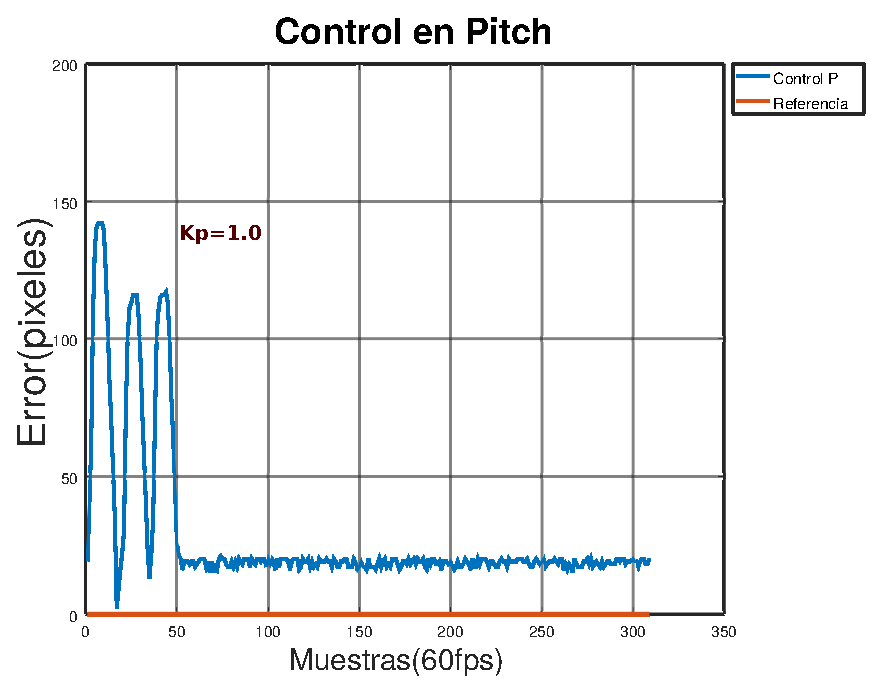
\includegraphics[width=0.83\textwidth]{Contenido/Cuerpo/Capitulo5/Fig25.eps}
	\captionof{figure}{Gráfica del error en Pitch con ganancia Kp = 1}\label{Fig4}
\end{center}
Como abordó anteriormente las ganancias deseadas para el control PI se ubican por debajo de cero, por lo que la siguiente prueba fue bajar la ganancia Kp.
La figura 5.19 muestra la respuesta del sistema con un controlador proporcional con ganancia Kp = 0.5
\begin{center}
	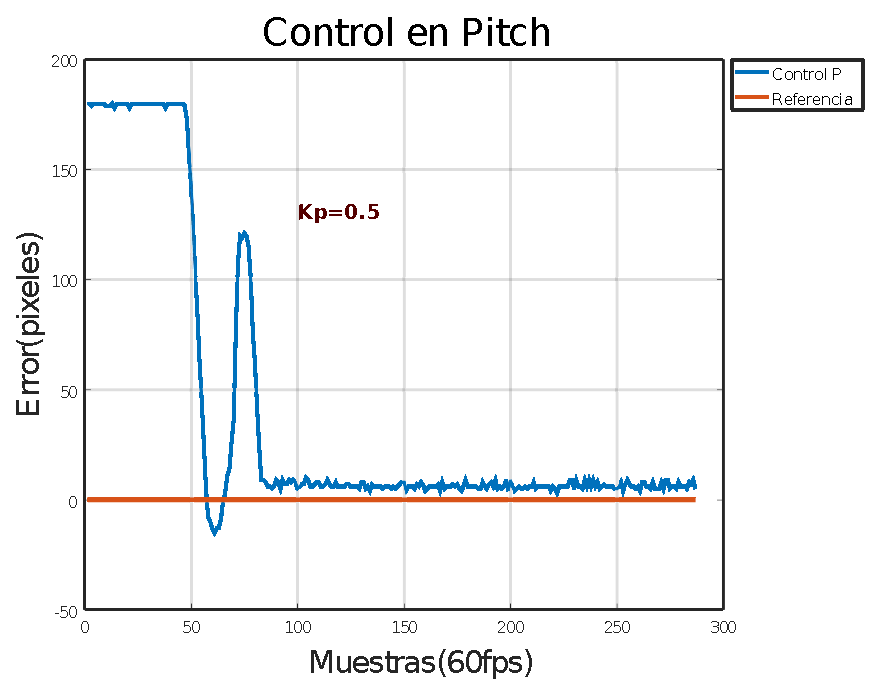
\includegraphics[width=0.8\textwidth]{Contenido/Cuerpo/Capitulo5/Fig26.eps}
	\captionof{figure}{Gráfica del error en Pitch con ganancia Kp = 0.5}\label{Fig4}
\end{center}
Las oscilaciones antes de que se mantenga estable fueron menores en comparación con ganancia Kp, por lo que, el valor de la ganancia se 
redujo a 0.35, obteniendo como resultado la figura 5.20 
\begin{center}
	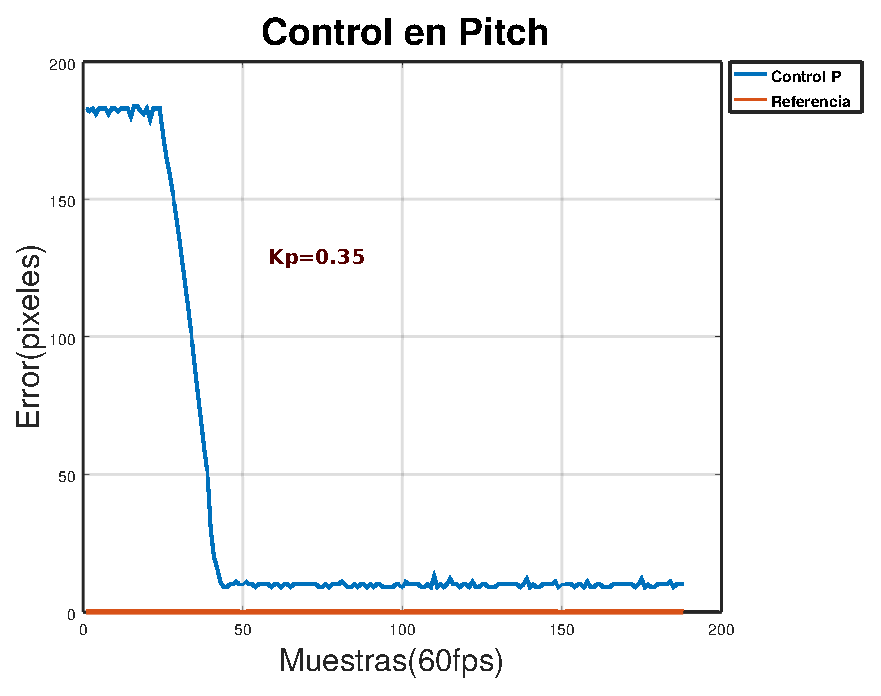
\includegraphics[width=0.8\textwidth]{Contenido/Cuerpo/Capitulo5/Fig27.eps}
	\captionof{figure}{Gráfica del error en Pitch con ganancia Kp = 0.35}\label{Fig4}
\end{center}
Es claro que en la gráfica 5.20 el sobre impulso es menor al 2\% sin embargo el error no converge a cero, se mantiene en 10, esto se
puede solucionar con un control Integral, reducir el error en estado estacionario agregando la suma de los errores multiplicada por una ganancia
Ki. Finalmante la gráfica de la figura 5.21 muestra el resultado de agregar un controlador PI a la planta en Pitch, donde el error en estado
estacionario es eliminado por la ganancia Ki, que a su vez ayuda a que el sistema converge en menor tiempo, donde se cumple una condición de diseño de $T_s = 0.2s$.
\begin{center}
	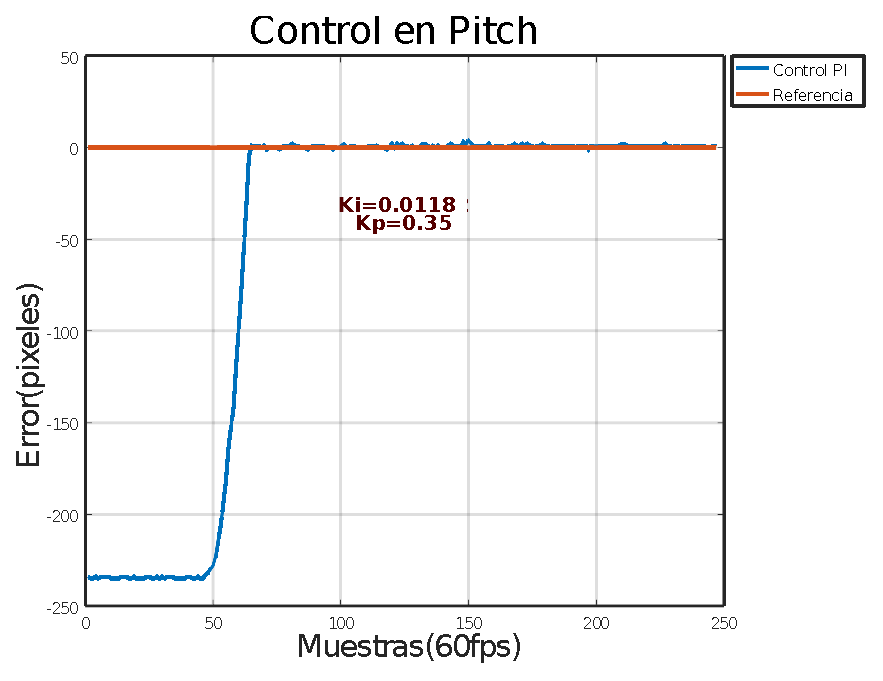
\includegraphics[width=0.8\textwidth]{Contenido/Cuerpo/Capitulo5/Fig28.eps}
	\captionof{figure}{Gráfica del error en Pitch con control PI}\label{Fig4}
\end{center}

\subsection{Control en Yaw}
El sistema dinámico en Yaw es de primer orden, la obtención de la ecuación diferencial
fue obtenida en el capítulo 3, de donde se obtuvo
\begin{equation}
	J_k\dot{r}_k = T_z+T_D
\end{equation}
Pasando la ecuación 5.21 al dominio de Laplace obtenemos
\begin{equation}
	J_{k}SR_k(s) = T_z(s)
\end{equation}
Dividimos entrada sobre salida, o en otras palabras, obtenemos la función de transferencia en lazo abierto
\begin{equation}
	G = \frac{R_k(s)}{T_z(s)} =  \frac{1}{J_{k}s}
\end{equation}
Y en lazo cerrado la ecuación 5.22 se transforma en 5.23 
\begin{equation}
	G_c = \frac{G}{1 +GH} = \frac{1}{J_{k}s+1}
\end{equation}
Donde \\
$J_k = J_{kz} + J_{az} $ 
La figura 5.22 es el resultado de la simulación del sistema dinámico de pitch en lazo cerrado ante una entrada escalón.
\begin{center}
	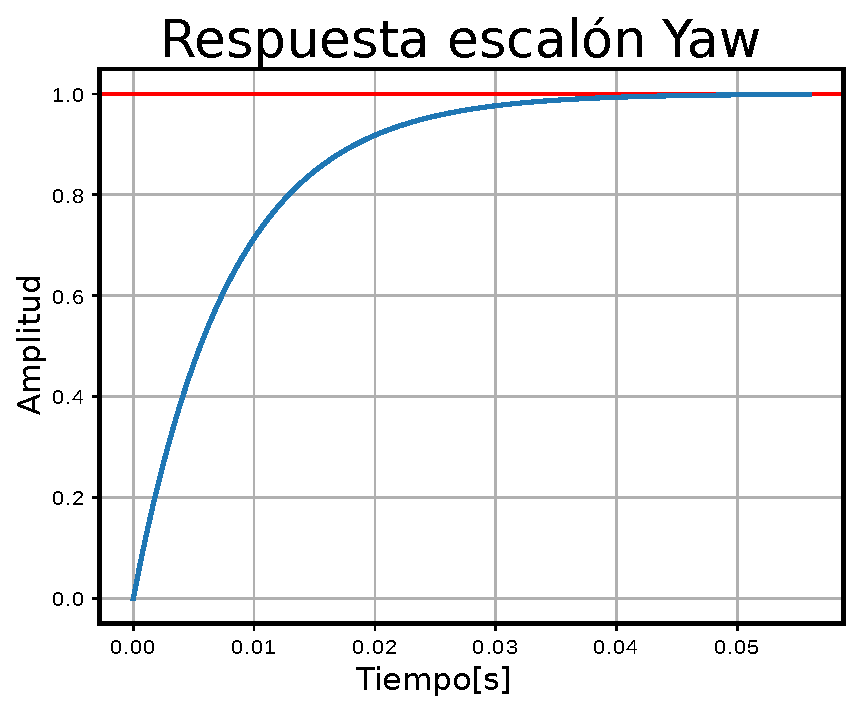
\includegraphics[width=0.6\textwidth]{Contenido/Cuerpo/Capitulo5/Fig39.eps}
	\captionof{figure}{Simulación entrada escalón para yaw}\label{Fig4}
\end{center}
Los valores para la ecuación 5.30 se obtuvieron del trabajo de \cite{Paper::Abdo2013}, debido a la similitud del sistema físico, donde
$J_{k} = 0.008$
De manera similar que en pitch tenemos un sistema de lazo cerrado donde se involucra el lazo de control del
servomotor y la retroalimentación en la cámara como se observa en la figura 5.23
\begin{center}
	\includegraphics[width=0.95\textwidth]{Contenido/Cuerpo/Capitulo5/Fig34.eps}
	\captionof{figure}{Lazo de control para Yaw}\label{Fig4}
\end{center}
\subsubsection{Diseño de control}
De manera similar que en el control de Pitch en Yaw se diseñó un control PI debido a que dichos sistemas comparten comportamiento similar y se modelaron como sistemas de primer orden.
Para este sistema los parámetros de diseño son los siguientes
\begin{itemize}
	\item $T_s$ = 0.3s
	\item Error menor al 2\%
	\item El máximo sobre impulso no sobre pasa del 2\%
\end{itemize}
El procedimiento es el mismo que se abordó al diseñar el control para pitch, por lo que solo se agregan puntos claves del proceso.
La función de transferencia deseada se satisface las condiciones de diseño está dada por la expresión 5.25
\begin{equation}
	G_d = \frac{482.7}{s^2 + 40s + 482.7}
\end{equation}
Donde los polos de la ecuación característica se sitúan en $-20 \pm 9.0958j$\\
Después de calcular la ganancia $K_p$ y el tiempo $T_i$ con base en los polos deseados, obtenemos la función de trasferencia(ecuación 5.26)
\begin{equation}
	G_c = 0.312 + \frac{3.8623}{s}
\end{equation}
Aplicando el lazo cerrado de la figura 5.15 y aplicando una entrada escalón se simuló la respuesta en el tiempo de la planta y el control.
\begin{center}
	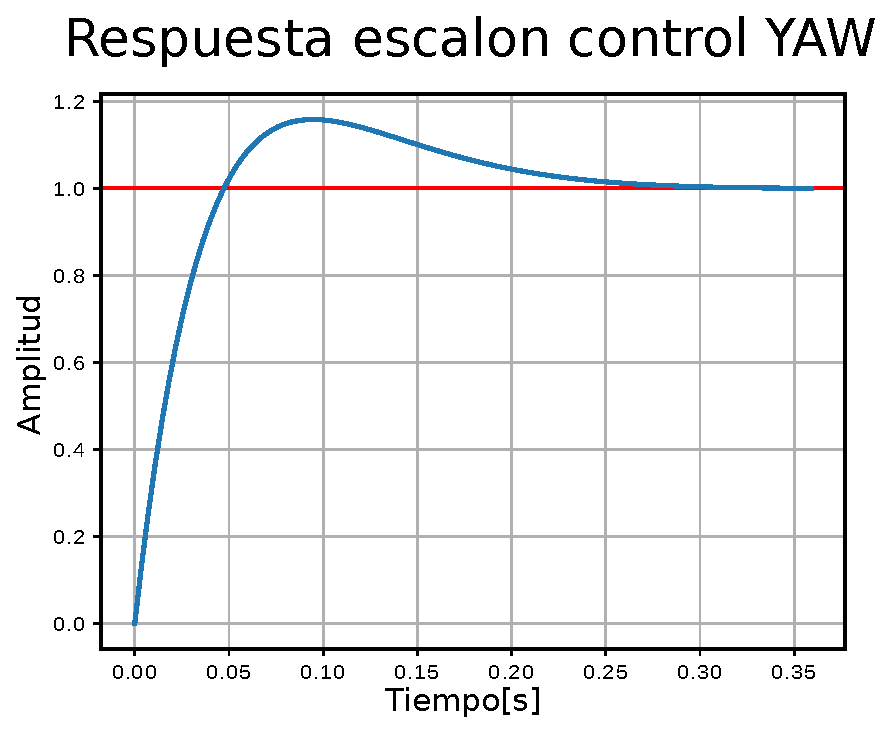
\includegraphics[width=0.65\textwidth]{Contenido/Cuerpo/Capitulo5/Fig40.eps}
	\captionof{figure}{Simulación del control PI en Yaw}\label{Fig4}
\end{center}
En la figura 5.24 podemos observar que el sistema simulado llega a la referencia en 0.3 segundos. Las ganancias que hacen que el sistema se comporte con los polos deseados son
$K_p = 0.312$ y $K_i = 0.06179$\\
El controlador sigue el mismo algoritmo descrito en el diagrama 5.17
\subsubsection{Sintonización de control}
Para sintonizar el control PI primero se aplica ganancia Kp y se observa el comportamiento del sistema, este
método nos ayuda a llegar lo más cerca a la referencia, que en este caso es cero, ya que estamos controlando
respecto a la dinámica del error.
\begin{center}
	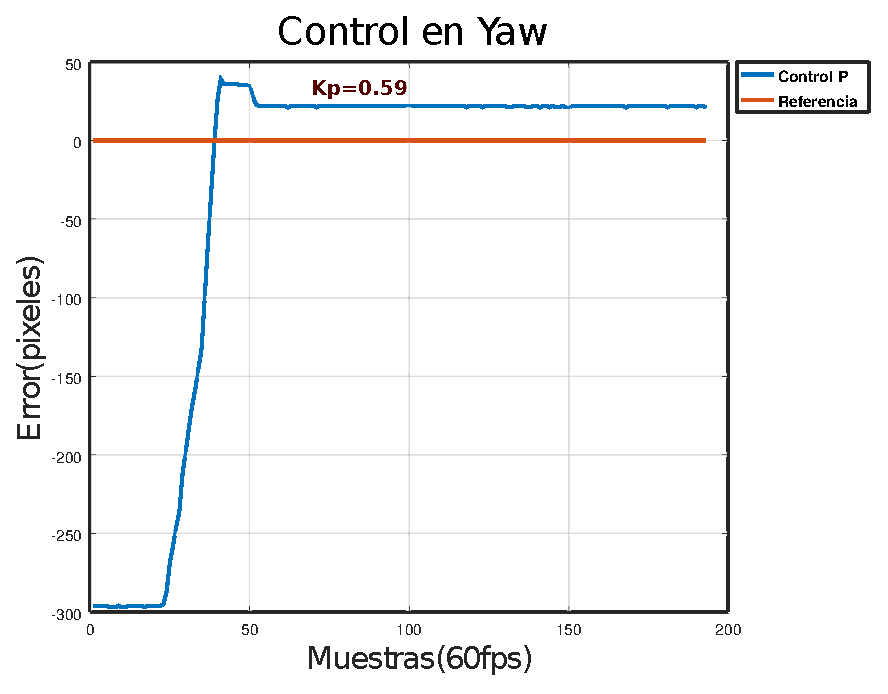
\includegraphics[width=0.75\textwidth]{Contenido/Cuerpo/Capitulo5/Fig30.eps}
	\captionof{figure}{Gráfica del error en Yaw con ganancia Kp = 0.59}\label{Fig4}
\end{center}
La figura 5.25 muestra un control proporcional con ganancia mayor al 0.5, hay un sobre impulso que posteriormente
hace que el sistema se mantenga con un error en 20 píxeles, le toma al sistema llegar a la referencia en 10 tiempos de
muestreo, pero el control no se mantiene en error cero. Con base en la ganancia obtenida en la etapa de diseño del control la ganancia proporcional debe estar por debajo de 0.5.
\begin{center}
	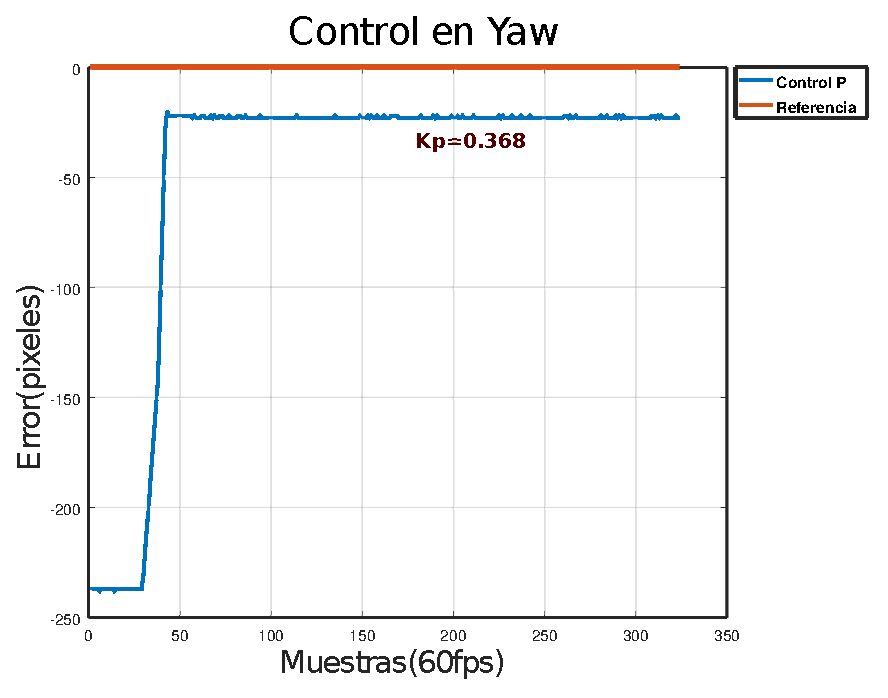
\includegraphics[width=0.74\textwidth]{Contenido/Cuerpo/Capitulo5/Fig31.eps}
	\captionof{figure}{Gráfica del error en Yaw con ganancia Kp = 0.368}\label{Fig4}
\end{center}
Ahora la ganancia es menor que 0.5, lo que hace que el sistema no tenga un sobre impulso, pero tampoco llega
a la referencia, se mantiene en un error de aproximadamente -20 píxeles, lo que tampoco es un comportamiento deseado.
La ganancia en 0.44 hace que el error se mantenga cercano a cero (figura 5.24), con lo cual podemos aplicar la ganancia integral para erradicar el error en estado estacionario. 
\begin{center}
	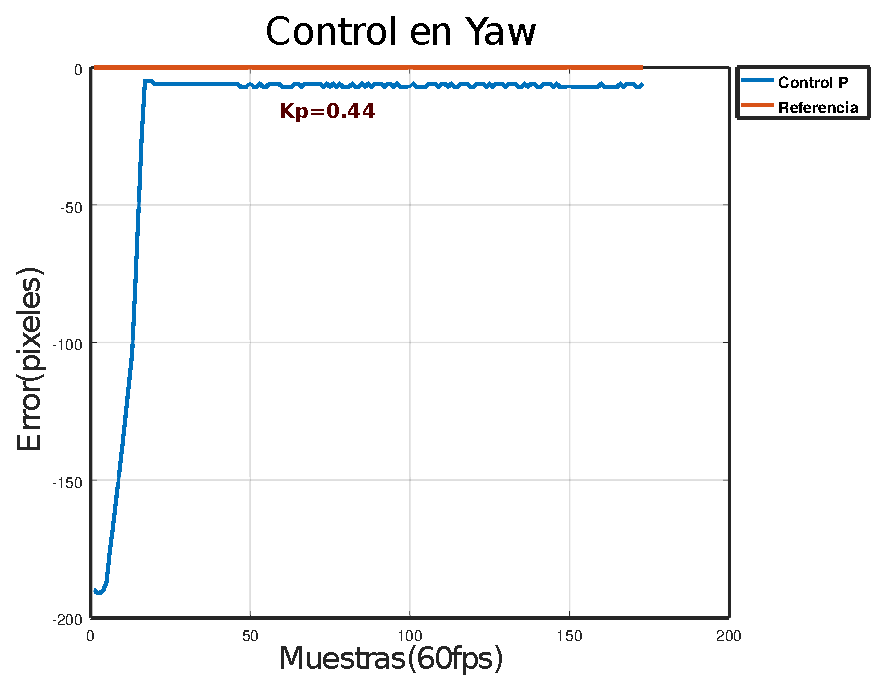
\includegraphics[width=0.83\textwidth]{Contenido/Cuerpo/Capitulo5/Fig32.eps}
	\captionof{figure}{Grafica del error en Yaw con ganancia Kp = 0.44}\label{Fig4}
\end{center}
Con una ganancia integral de 0.0351 el sistema se comporta como las especificaciones de diseño marcan, llegar a la referencia y mantenerse estable le toma al sistema 16 tiempos de
muestreo, que equivalen a 0.3s y además el sobre impulso se ubica en menos del 2\% por lo que podemos decir que el control satisface los requerimientos.
\begin{center}
	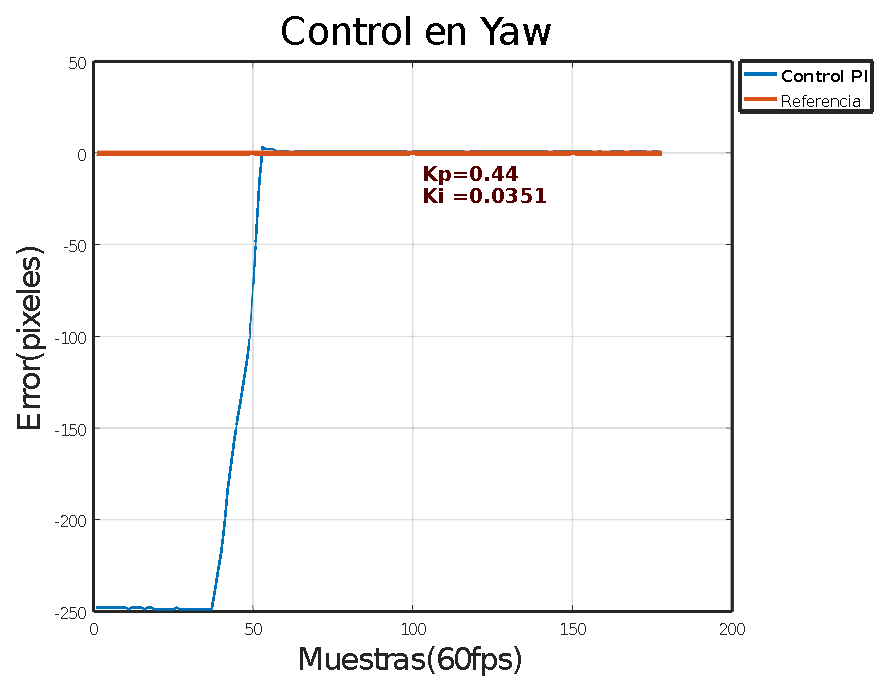
\includegraphics[width=0.83\textwidth]{Contenido/Cuerpo/Capitulo5/Fig33.eps}
	\captionof{figure}{Gráfica del error en Yaw con control PI}\label{Fig4}
\end{center}